\documentclass[]{article}
\usepackage{lmodern}
\usepackage{amssymb,amsmath}
\usepackage{ifxetex,ifluatex}
\usepackage{fixltx2e} % provides \textsubscript
\ifnum 0\ifxetex 1\fi\ifluatex 1\fi=0 % if pdftex
  \usepackage[T1]{fontenc}
  \usepackage[utf8]{inputenc}
\else % if luatex or xelatex
  \ifxetex
    \usepackage{mathspec}
    \usepackage{xltxtra,xunicode}
  \else
    \usepackage{fontspec}
  \fi
  \defaultfontfeatures{Mapping=tex-text,Scale=MatchLowercase}
  \newcommand{\euro}{€}
\fi
% use upquote if available, for straight quotes in verbatim environments
\IfFileExists{upquote.sty}{\usepackage{upquote}}{}
% use microtype if available
\IfFileExists{microtype.sty}{%
\usepackage{microtype}
\UseMicrotypeSet[protrusion]{basicmath} % disable protrusion for tt fonts
}{}
\usepackage[margin=1in]{geometry}
\ifxetex
  \usepackage[setpagesize=false, % page size defined by xetex
              unicode=false, % unicode breaks when used with xetex
              xetex]{hyperref}
\else
  \usepackage[unicode=true]{hyperref}
\fi
\hypersetup{breaklinks=true,
            bookmarks=true,
            pdfauthor={FEDORU},
            pdftitle={Enquête logiciels SU - Septembre 2015},
            colorlinks=true,
            citecolor=blue,
            urlcolor=blue,
            linkcolor=magenta,
            pdfborder={0 0 0}}
\urlstyle{same}  % don't use monospace font for urls
\usepackage{color}
\usepackage{fancyvrb}
\newcommand{\VerbBar}{|}
\newcommand{\VERB}{\Verb[commandchars=\\\{\}]}
\DefineVerbatimEnvironment{Highlighting}{Verbatim}{commandchars=\\\{\}}
% Add ',fontsize=\small' for more characters per line
\usepackage{framed}
\definecolor{shadecolor}{RGB}{248,248,248}
\newenvironment{Shaded}{\begin{snugshade}}{\end{snugshade}}
\newcommand{\KeywordTok}[1]{\textcolor[rgb]{0.13,0.29,0.53}{\textbf{{#1}}}}
\newcommand{\DataTypeTok}[1]{\textcolor[rgb]{0.13,0.29,0.53}{{#1}}}
\newcommand{\DecValTok}[1]{\textcolor[rgb]{0.00,0.00,0.81}{{#1}}}
\newcommand{\BaseNTok}[1]{\textcolor[rgb]{0.00,0.00,0.81}{{#1}}}
\newcommand{\FloatTok}[1]{\textcolor[rgb]{0.00,0.00,0.81}{{#1}}}
\newcommand{\ConstantTok}[1]{\textcolor[rgb]{0.00,0.00,0.00}{{#1}}}
\newcommand{\CharTok}[1]{\textcolor[rgb]{0.31,0.60,0.02}{{#1}}}
\newcommand{\SpecialCharTok}[1]{\textcolor[rgb]{0.00,0.00,0.00}{{#1}}}
\newcommand{\StringTok}[1]{\textcolor[rgb]{0.31,0.60,0.02}{{#1}}}
\newcommand{\VerbatimStringTok}[1]{\textcolor[rgb]{0.31,0.60,0.02}{{#1}}}
\newcommand{\SpecialStringTok}[1]{\textcolor[rgb]{0.31,0.60,0.02}{{#1}}}
\newcommand{\ImportTok}[1]{{#1}}
\newcommand{\CommentTok}[1]{\textcolor[rgb]{0.56,0.35,0.01}{\textit{{#1}}}}
\newcommand{\DocumentationTok}[1]{\textcolor[rgb]{0.56,0.35,0.01}{\textbf{\textit{{#1}}}}}
\newcommand{\AnnotationTok}[1]{\textcolor[rgb]{0.56,0.35,0.01}{\textbf{\textit{{#1}}}}}
\newcommand{\CommentVarTok}[1]{\textcolor[rgb]{0.56,0.35,0.01}{\textbf{\textit{{#1}}}}}
\newcommand{\OtherTok}[1]{\textcolor[rgb]{0.56,0.35,0.01}{{#1}}}
\newcommand{\FunctionTok}[1]{\textcolor[rgb]{0.00,0.00,0.00}{{#1}}}
\newcommand{\VariableTok}[1]{\textcolor[rgb]{0.00,0.00,0.00}{{#1}}}
\newcommand{\ControlFlowTok}[1]{\textcolor[rgb]{0.13,0.29,0.53}{\textbf{{#1}}}}
\newcommand{\OperatorTok}[1]{\textcolor[rgb]{0.81,0.36,0.00}{\textbf{{#1}}}}
\newcommand{\BuiltInTok}[1]{{#1}}
\newcommand{\ExtensionTok}[1]{{#1}}
\newcommand{\PreprocessorTok}[1]{\textcolor[rgb]{0.56,0.35,0.01}{\textit{{#1}}}}
\newcommand{\AttributeTok}[1]{\textcolor[rgb]{0.77,0.63,0.00}{{#1}}}
\newcommand{\RegionMarkerTok}[1]{{#1}}
\newcommand{\InformationTok}[1]{\textcolor[rgb]{0.56,0.35,0.01}{\textbf{\textit{{#1}}}}}
\newcommand{\WarningTok}[1]{\textcolor[rgb]{0.56,0.35,0.01}{\textbf{\textit{{#1}}}}}
\newcommand{\AlertTok}[1]{\textcolor[rgb]{0.94,0.16,0.16}{{#1}}}
\newcommand{\ErrorTok}[1]{\textcolor[rgb]{0.64,0.00,0.00}{\textbf{{#1}}}}
\newcommand{\NormalTok}[1]{{#1}}
\usepackage{graphicx,grffile}
\makeatletter
\def\maxwidth{\ifdim\Gin@nat@width>\linewidth\linewidth\else\Gin@nat@width\fi}
\def\maxheight{\ifdim\Gin@nat@height>\textheight\textheight\else\Gin@nat@height\fi}
\makeatother
% Scale images if necessary, so that they will not overflow the page
% margins by default, and it is still possible to overwrite the defaults
% using explicit options in \includegraphics[width, height, ...]{}
\setkeys{Gin}{width=\maxwidth,height=\maxheight,keepaspectratio}
\setlength{\parindent}{0pt}
\setlength{\parskip}{6pt plus 2pt minus 1pt}
\setlength{\emergencystretch}{3em}  % prevent overfull lines
\providecommand{\tightlist}{%
  \setlength{\itemsep}{0pt}\setlength{\parskip}{0pt}}
\setcounter{secnumdepth}{5}

%%% Use protect on footnotes to avoid problems with footnotes in titles
\let\rmarkdownfootnote\footnote%
\def\footnote{\protect\rmarkdownfootnote}

%%% Change title format to be more compact
\usepackage{titling}

% Create subtitle command for use in maketitle
\newcommand{\subtitle}[1]{
  \posttitle{
    \begin{center}\large#1\end{center}
    }
}

\setlength{\droptitle}{-2em}
  \title{Enquête logiciels SU - Septembre 2015}
  \pretitle{\vspace{\droptitle}\centering\huge}
  \posttitle{\par}
  \author{FEDORU}
  \preauthor{\centering\large\emph}
  \postauthor{\par}
  \predate{\centering\large\emph}
  \postdate{\par}
  \date{07/09/2015}


% Redefines (sub)paragraphs to behave more like sections
\ifx\paragraph\undefined\else
\let\oldparagraph\paragraph
\renewcommand{\paragraph}[1]{\oldparagraph{#1}\mbox{}}
\fi
\ifx\subparagraph\undefined\else
\let\oldsubparagraph\subparagraph
\renewcommand{\subparagraph}[1]{\oldsubparagraph{#1}\mbox{}}
\fi

\begin{document}
\maketitle

{
\hypersetup{linkcolor=black}
\setcounter{tocdepth}{2}
\tableofcontents
}
Objectif: lesRPU sont produits par des ES disposant d'une autorisation
de SU. Les informations sont issues des données d'un patient, recueillis
par du personnel administratif, soignant et médical sur un logiciel mis
à disposition par le service informatique de l'établissement. Le
logiciel est fourni par un éditeur ou plus rarement développé localement
et administré par le service informatique de l'établissement hospitalier
(SIH). La qualité et l'exhaustivité des RPU dépend d'une chaine
d'intervenant. Un RPU est considéré comme crée s'il comporte la date et
heure d'entrée, le code postal, la commune et la date de naissance d'un
consultant (?).L'exhaustivité est la diffférence entre le nombre de RPU
produits pendant une période et le nombre de primo passage aux urgences
sur la même période. Il n'y a pas de référentiel absolu pour mesurer le
nombre de primo passages. Selon le cas il peut s'agir du nombre de RPU
eux-mêmes, du chiffre de la SAE, d'une mesure à partir du PMSI. La
qualité des RPU se mesure par l'écart entre la valeur attendue d'un item
et la réponse fournie. La réponse fournie peut être manquante ou non
conforme à un référentiel de valeur. Le référentiel s'appuie sur la
cahier des charges de l'INVS, sur des référentiels issus de sociétés
savantes (SFMU) ou sur des consenssus d'expert (FEDORU).

\section{Historique}\label{historique}

\begin{itemize}
\item
  7/9/2015 Reprise de l'exploitation des logiciels des SU

  \begin{itemize}
  \tightlist
  \item
    fichier source: DATA/FEDORU - ENQUETE LOGICIEL 2015 - V2 (12 06 15)
    (3)
  \item
    création d'un dossier spécifique \textbf{Septembre2015} contenent un
    sous dossier \textbf{data} pour y stocker les résultats régionaux
    sous forme de fichier .csv.
  \end{itemize}
\item
  17/9/2015 récup données ORUMIP (Olivier Azema)
\item
  18/9/2015 données Bourgogne mises à jour
\item
  30/9/2015 intégration des données de la Franche-comté
\item
  13/10/2015 intégration de la Lorraine
\end{itemize}

\subsection{Récupération des fichiers
csv}\label{recuperation-des-fichiers-csv}

\begin{verbatim}
[1] "alsace.csv"
[1] "alsace.csv~"
[1] "aquitaine.csv"
[1] "bourgogne.csv"
[1] "bretagne.csv"
[1] "champagne.csv"
[1] "franche_comte.csv"
[1] "limousin.csv"
[1] "lorraine2.csv"
[1] "midipy.csv"
[1] "ORUMIP.csv"
[1] "paca.csv"
[1] "rhone.csv"
\end{verbatim}

\begin{verbatim}
[1] "/Users/jcb/Documents/FEDORU/InformatisationSU/Septembre2015"
\end{verbatim}

\section{Données générales}\label{donnees-generales}

Périmètre du questionnaire:

\begin{itemize}
\tightlist
\item
  période: 1er janvier 2015 au 31 mars 2015 (1er trimestre)
\item
  concerne toutes les structures volontaires membres de la FEDORU.
  Coordination régionale assurée par les ORU
\item
  questions
\end{itemize}

\subsection{Résultats}\label{resultats}

\begin{itemize}
\tightlist
\item
  Nombre de régions participantes: 11:
\end{itemize}

\begin{verbatim}
 [1] "ALSACE"             "AQUITAINE"          "BOURGOGNE"          "BRETAGNE"          
 [5] "CHAMPAGNE ARDENNES" "FRANCHE COMTE"      "LIMOUSIN"           "LORRAINE"          
 [9] "MIDI PYRENEES"      "PACA"               "RHONE ALPES"       
\end{verbatim}

\begin{itemize}
\tightlist
\item
  Nombre de sites concernés: 316
\end{itemize}

\section{Cartographie}\label{cartographie}

Cartographie des régions participantes et des logiciels.

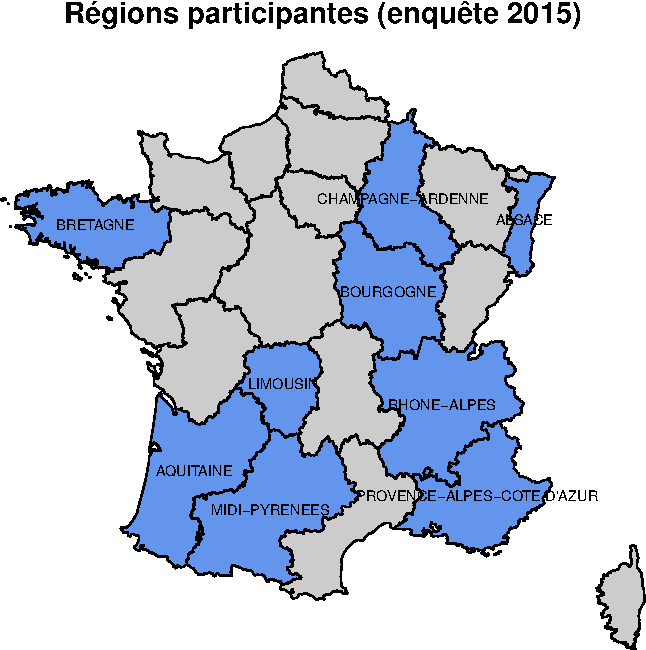
\includegraphics{septembre2015_files/figure-latex/carto_region-1.pdf}

Régions participantes à l'étude

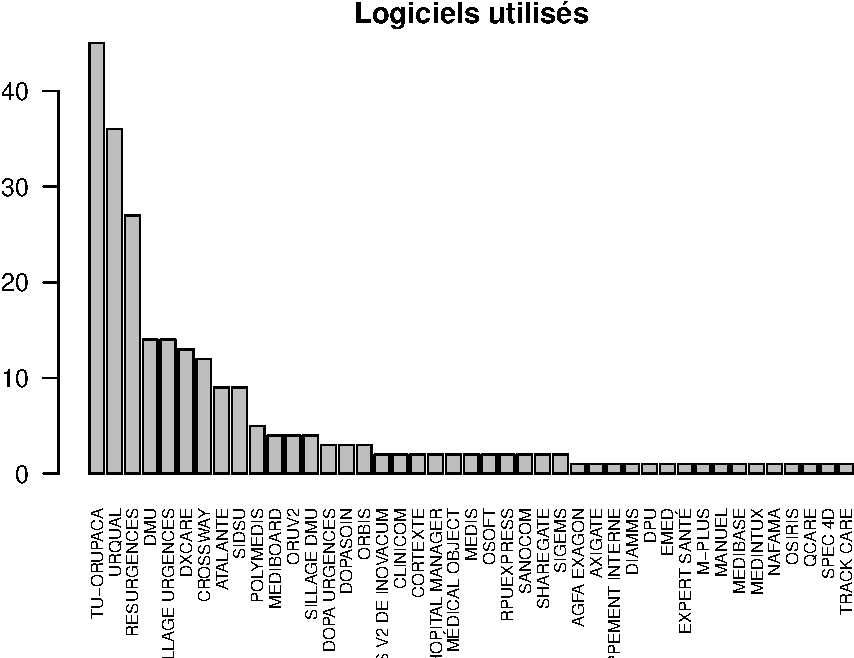
\includegraphics{septembre2015_files/figure-latex/unnamed-chunk-4-1.pdf}

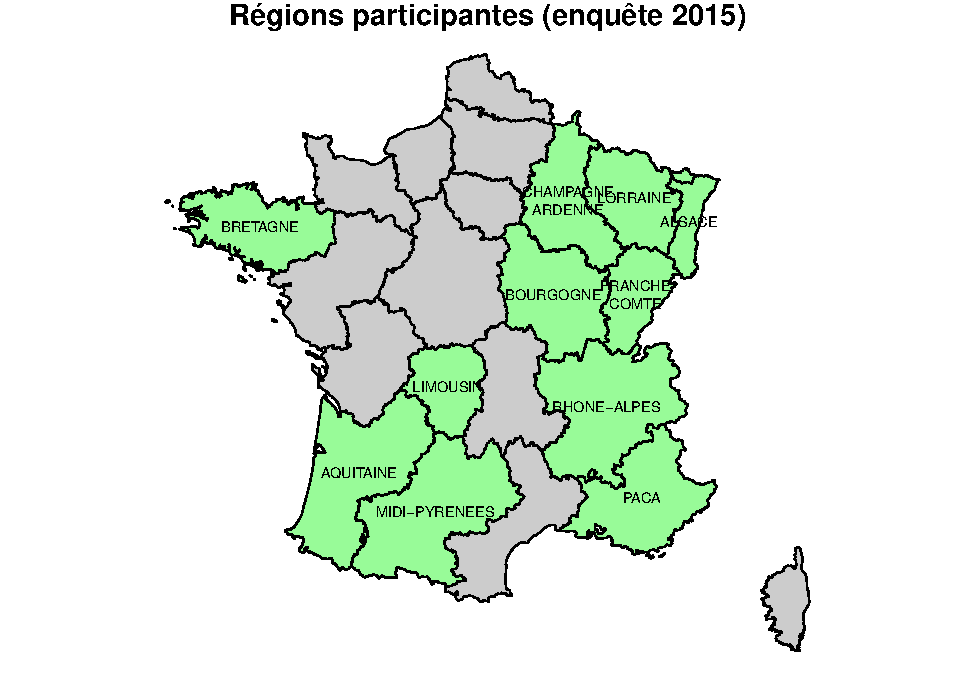
\includegraphics{septembre2015_files/figure-latex/unnamed-chunk-5-1.pdf}
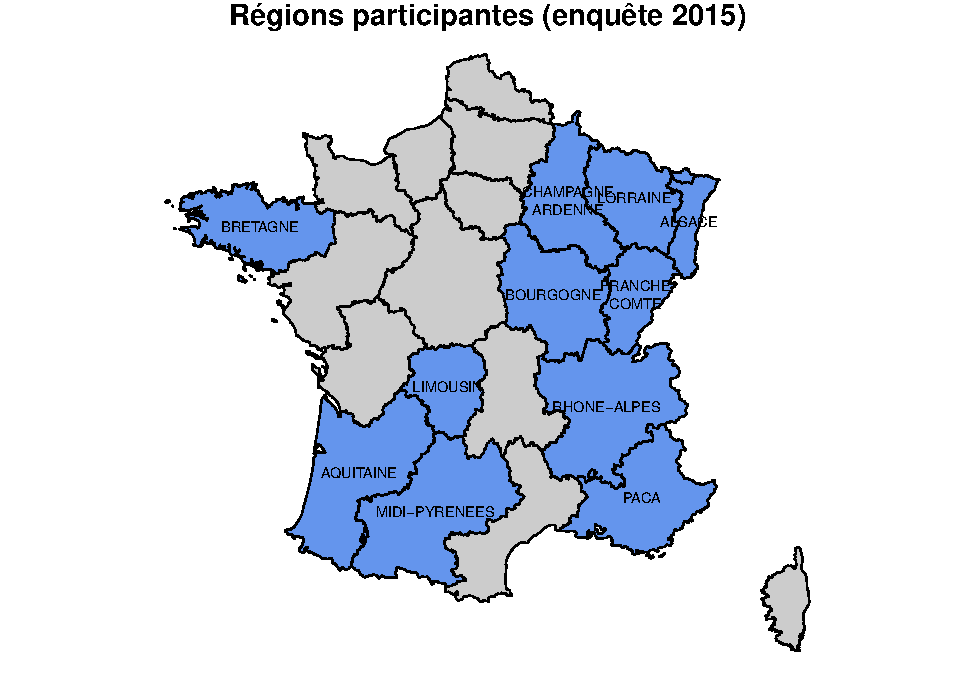
\includegraphics{septembre2015_files/figure-latex/unnamed-chunk-5-2.pdf}

\section{Editeurs}\label{editeurs}

\begin{itemize}
\tightlist
\item
  Dans la majorité des cas (79.03), les répondants ne connaissent pas
  leur éditeur.
\item
  Il en est de même pour la version: 63.44 \% des cas, la version n'est
  pas précisée.
\end{itemize}

\section{Logiciels 2015}\label{logiciels-2015}

\begin{itemize}
\tightlist
\item
  Nombre de logiciels utilisés: 53
\item
  Huit produits sont cités 10 fois ou plus.
\end{itemize}

\subsection{Logiciels par ordre
décroissant}\label{logiciels-par-ordre-decroissant}

\begin{verbatim}

                  DMU           RESURGENCES            TU-ORUPACA                URQUAL 
                   50                    47                    47                    40 
             CROSSWAY                DXCARE              ATALANTE             MEDIBOARD 
                   20                    18                    13                     9 
                SIDSU                 ORUV2      SILLAGE URGENCES              DOPASOIN 
                    9                     8                     8                     6 
             FIRSTNET                 ORBIS              CLINICOM             POLYMEDIS 
                    6                     6                     5                     5 
              ANTARES              CORTEXTE DEVELOPPEMENT INTERNE                   DPU 
                    4                     4                     4                     4 
       MÉDICAL OBJECT            RPUEXPRESS         DOPA URGENCES               EXAGONE 
                    4                     4                     3                     3 
         EXPERT SANTE              EXPERTIZ                SIGEMS                DIAMMS 
                    3                     3                     3                     2 
              DX CARE                  EMED               H+ACUTE       HOPITAL MANAGER 
                    2                     2                     2                     2 
               OSIRIS                 OSOFT               SANOCOM             SHAREGATE 
                    2                     2                     2                     2 
          SILLAGE DMU               AXIGATE                CLIMCO          CORA URGENCE 
                    2                     1                     1                     1 
               CORPUS              E SHERPA              EQUAFILE                M-PLUS 
                    1                     1                     1                     1 
             MEDIBASE              MEDINTUX                 MEDIS              MEDIWERE 
                    1                     1                     1                     1 
               NAFAMA                 QCARE               SPEC 4D            TRACK CARE 
                    1                     1                     1                     1 
               URGEST 
                    1 
\end{verbatim}

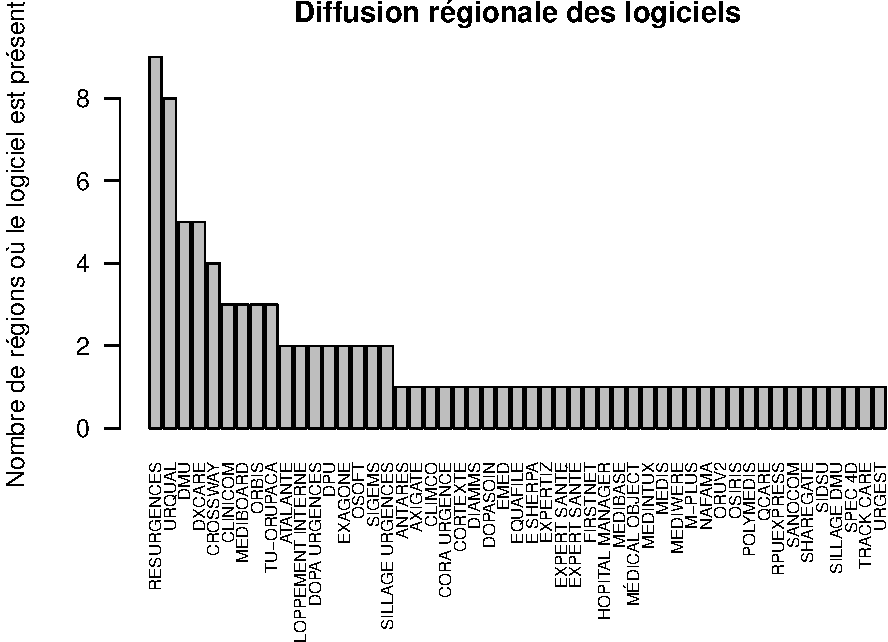
\includegraphics{septembre2015_files/figure-latex/unnamed-chunk-8-1.pdf}

Top Ten

\begin{Shaded}
\begin{Highlighting}[]
\KeywordTok{par}\NormalTok{(}\DataTypeTok{mar=}\KeywordTok{c}\NormalTok{(}\DecValTok{4}\NormalTok{,}\DecValTok{7}\NormalTok{,}\DecValTok{2}\NormalTok{,}\DecValTok{2}\NormalTok{))}
\NormalTok{t <-}\StringTok{ }\KeywordTok{sort}\NormalTok{(}\KeywordTok{table}\NormalTok{(d$Logiciel_2015), }\DataTypeTok{decreasing =} \OtherTok{TRUE}\NormalTok{)}
\NormalTok{t10 <-}\StringTok{ }\NormalTok{t[}\DecValTok{10}\NormalTok{:}\DecValTok{1}\NormalTok{]}
\KeywordTok{barplot}\NormalTok{(t10, }\DataTypeTok{horiz =} \OtherTok{TRUE}\NormalTok{, }\DataTypeTok{las =} \DecValTok{1}\NormalTok{, }\DataTypeTok{cex.names =} \FloatTok{0.7}\NormalTok{, }\DataTypeTok{main =} \StringTok{"Logiciels utilisés - Top 10"}\NormalTok{, }\DataTypeTok{col =} \KeywordTok{ifelse}\NormalTok{(t10 >}\StringTok{ }\DecValTok{9}\NormalTok{, }\StringTok{"cornflowerblue"}\NormalTok{, }\StringTok{"gray80"}\NormalTok{), }\DataTypeTok{xlab =} \StringTok{"Fréquence d'utilisation"}\NormalTok{)}
\end{Highlighting}
\end{Shaded}

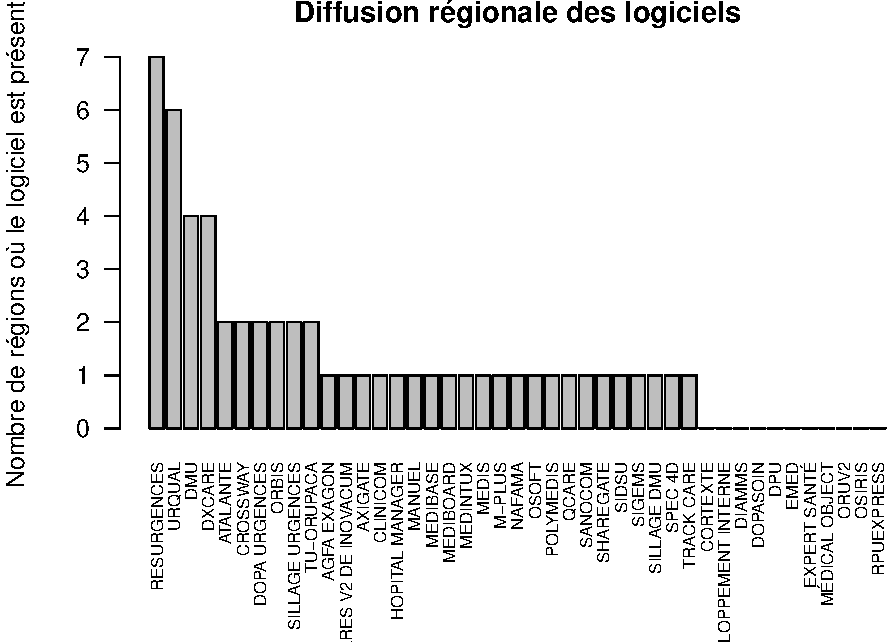
\includegraphics{septembre2015_files/figure-latex/unnamed-chunk-9-1.pdf}

\subsection{Logiciels par région}\label{logiciels-par-region}

\begin{verbatim}
                       
                        ALSACE AQUITAINE BOURGOGNE BRETAGNE CHAMPAGNE ARDENNES
  ANTARES                    4         0         0        0                  0
  ATALANTE                  11         0         2        0                  0
  AXIGATE                    0         1         0        0                  0
  CLIMCO                     0         0         0        0                  0
  CLINICOM                   2         0         0        0                  0
  CORA URGENCE               0         0         0        0                  0
  CORPUS                     0         0         0        0                  0
  CORTEXTE                   0         0         0        0                  0
  CROSSWAY                   0         3         3        0                  0
  DEVELOPPEMENT INTERNE      0         0         0        0                  0
  DIAMMS                     0         0         0        0                  0
  DMU                        2         0         7        0                  3
  DOPA URGENCES              0         1         0        0                  2
  DOPASOIN                   0         0         0        0                  0
  DPU                        0         0         0        0                  0
  DX CARE                    2         0         0        0                  0
  DXCARE                     4         6         1        0                  1
  E SHERPA                   0         0         0        0                  0
  EMED                       0         0         0        0                  0
  EQUAFILE                   0         0         0        0                  0
  EXAGONE                    0         0         1        0                  0
  EXPERT SANTE               0         0         0        0                  0
  EXPERTIZ                   0         0         0        0                  0
  FIRSTNET                   0         0         0        0                  0
  H+ACUTE                    0         0         0        0                  0
  HOPITAL MANAGER            0         0         2        0                  0
  M-PLUS                     0         1         0        0                  0
  MEDIBASE                   0         1         0        0                  0
  MEDIBOARD                  0         0         0        1                  0
  MÉDICAL OBJECT             0         0         0        0                  0
  MEDINTUX                   0         0         0        0                  0
  MEDIS                      0         0         0        1                  0
  MEDIWERE                   0         0         0        0                  0
  NAFAMA                     0         0         0        0                  1
  ORBIS                      2         0         0        1                  0
  ORUV2                      0         0         0        0                  0
  OSIRIS                     0         0         0        0                  0
  OSOFT                      0         0         0        1                  0
  POLYMEDIS                  0         0         0        0                  5
  QCARE                      0         0         0        0                  0
  RESURGENCES                2         1         3        7                  1
  RPUEXPRESS                 0         0         0        0                  0
  SANOCOM                    0         2         0        0                  0
  SHAREGATE                  0         2         0        0                  0
  SIDSU                      0         9         0        0                  0
  SIGEMS                     0         2         0        0                  0
  SILLAGE DMU                0         0         0        2                  0
  SILLAGE URGENCES           0         2         0        6                  0
  SPEC 4D                    0         0         0        0                  0
  TRACK CARE                 0         1         0        0                  0
  TU-ORUPACA                 0         0         1        0                  0
  URGEST                     0         0         0        0                  0
  URQUAL                     0         3         3       11                  3
                       
                        FRANCHE COMTE LIMOUSIN LORRAINE MIDI PYRENEES PACA RHONE ALPES
  ANTARES                           0        0        0             0    0           0
  ATALANTE                          0        0        0             0    0           0
  AXIGATE                           0        0        0             0    0           0
  CLIMCO                            0        0        0             0    0           1
  CLINICOM                          0        0        0             2    0           1
  CORA URGENCE                      0        0        0             0    0           1
  CORPUS                            0        0        1             0    0           0
  CORTEXTE                          0        0        0             4    0           0
  CROSSWAY                          1        0        1            12    0           0
  DEVELOPPEMENT INTERNE             0        0        0             2    0           2
  DIAMMS                            0        0        0             2    0           0
  DMU                               0        0        0             0    2          36
  DOPA URGENCES                     0        0        0             0    0           0
  DOPASOIN                          0        0        0             6    0           0
  DPU                               0        0        0             2    0           2
  DX CARE                           0        0        0             0    0           0
  DXCARE                            0        0        2             4    0           0
  E SHERPA                          0        0        0             0    0           1
  EMED                              0        0        0             2    0           0
  EQUAFILE                          1        0        0             0    0           0
  EXAGONE                           0        0        0             0    0           2
  EXPERT SANTE                      0        0        0             2    0           1
  EXPERTIZ                          0        0        0             0    0           3
  FIRSTNET                          6        0        0             0    0           0
  H+ACUTE                           0        0        2             0    0           0
  HOPITAL MANAGER                   0        0        0             0    0           0
  M-PLUS                            0        0        0             0    0           0
  MEDIBASE                          0        0        0             0    0           0
  MEDIBOARD                         0        0        0             4    0           4
  MÉDICAL OBJECT                    0        0        0             4    0           0
  MEDINTUX                          0        0        0             0    1           0
  MEDIS                             0        0        0             0    0           0
  MEDIWERE                          0        0        0             0    0           1
  NAFAMA                            0        0        0             0    0           0
  ORBIS                             0        0        0             0    0           3
  ORUV2                             0        0        0             8    0           0
  OSIRIS                            0        0        0             2    0           0
  OSOFT                             0        0        0             0    0           1
  POLYMEDIS                         0        0        0             0    0           0
  QCARE                             0        0        0             0    1           0
  RESURGENCES                       5        6       17             0    2           3
  RPUEXPRESS                        0        0        0             4    0           0
  SANOCOM                           0        0        0             0    0           0
  SHAREGATE                         0        0        0             0    0           0
  SIDSU                             0        0        0             0    0           0
  SIGEMS                            0        0        0             0    0           1
  SILLAGE DMU                       0        0        0             0    0           0
  SILLAGE URGENCES                  0        0        0             0    0           0
  SPEC 4D                           0        1        0             0    0           0
  TRACK CARE                        0        0        0             0    0           0
  TU-ORUPACA                        0        0        0             4   42           0
  URGEST                            0        0        0             0    0           1
  URQUAL                            0        2        0            10    2           6
\end{verbatim}

Nombre de logiciels différents par région

\begin{verbatim}
            ALSACE          AQUITAINE          BOURGOGNE           BRETAGNE 
                 8                 14                  9                  8 
CHAMPAGNE ARDENNES      FRANCHE COMTE           LIMOUSIN           LORRAINE 
                 7                  4                  3                  5 
     MIDI PYRENEES               PACA        RHONE ALPES 
                17                  6                 18 
\end{verbatim}

Nombre de logiciels différents par rapport au nombre de SU de la région

\begin{verbatim}

              PACA           LORRAINE      MIDI PYRENEES        RHONE ALPES 
              0.12               0.22               0.23               0.26 
          BRETAGNE             ALSACE      FRANCHE COMTE           LIMOUSIN 
              0.27               0.28               0.31               0.33 
         BOURGOGNE          AQUITAINE CHAMPAGNE ARDENNES 
              0.39               0.40               0.44 
\end{verbatim}

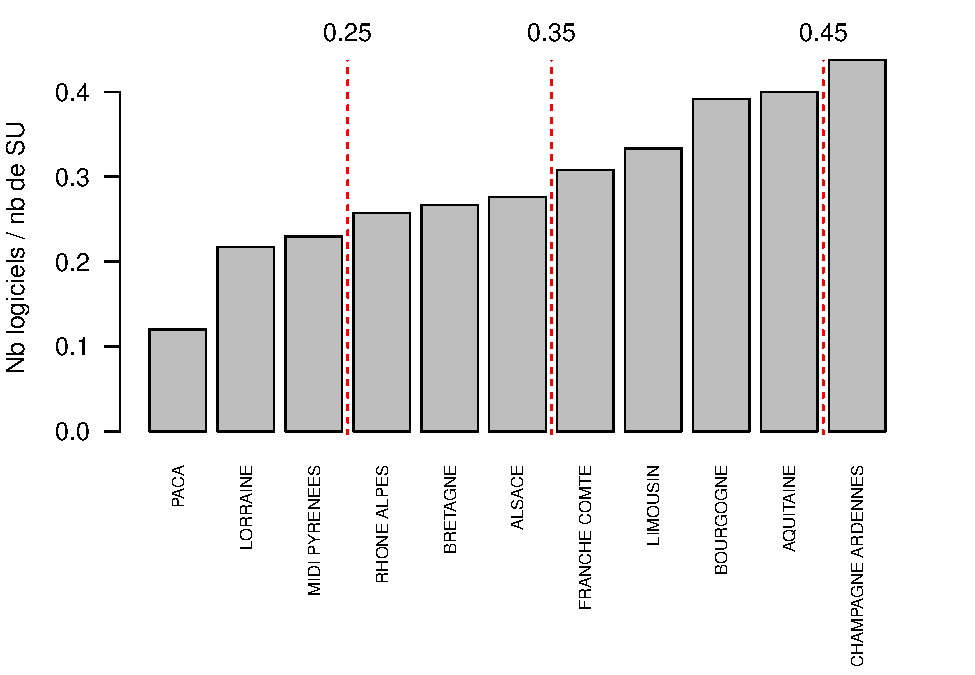
\includegraphics{septembre2015_files/figure-latex/unnamed-chunk-12-1.pdf}

\subsection{Cartographie des
logiciels}\label{cartographie-des-logiciels}

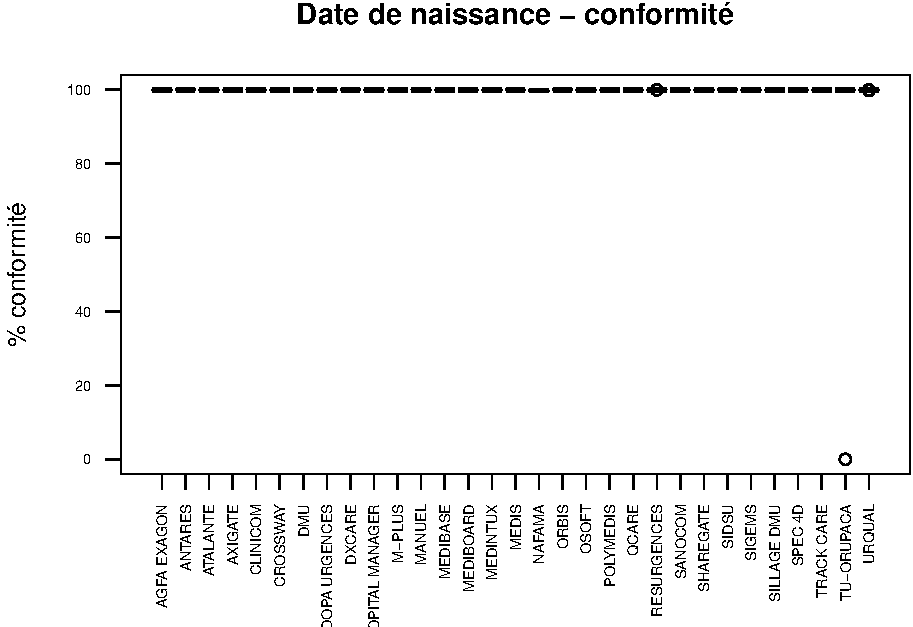
\includegraphics{septembre2015_files/figure-latex/unnamed-chunk-13-1.pdf}

\subsection{Un logiciel est présent dans combien de régions
?}\label{un-logiciel-est-present-dans-combien-de-regions}

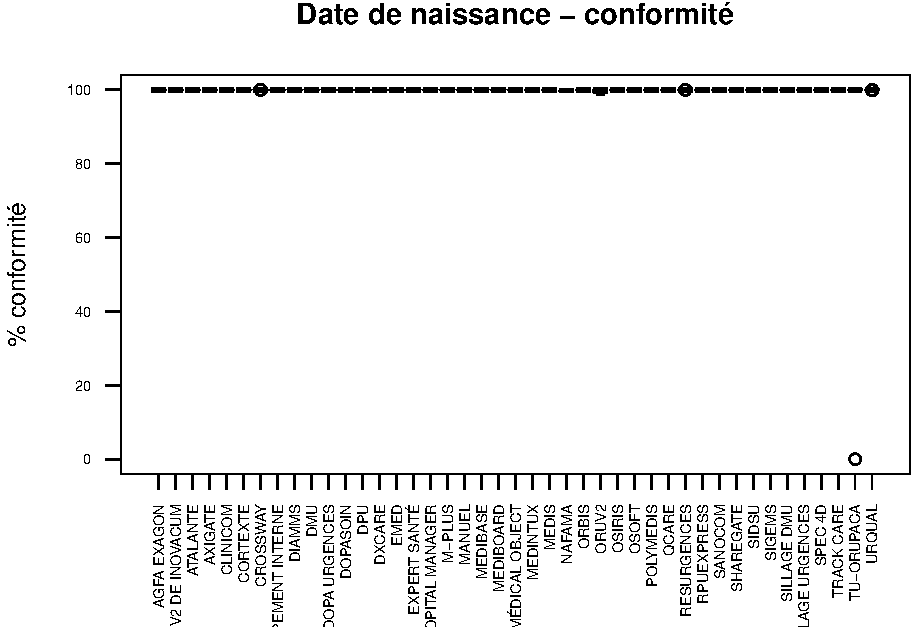
\includegraphics{septembre2015_files/figure-latex/unnamed-chunk-14-1.pdf}
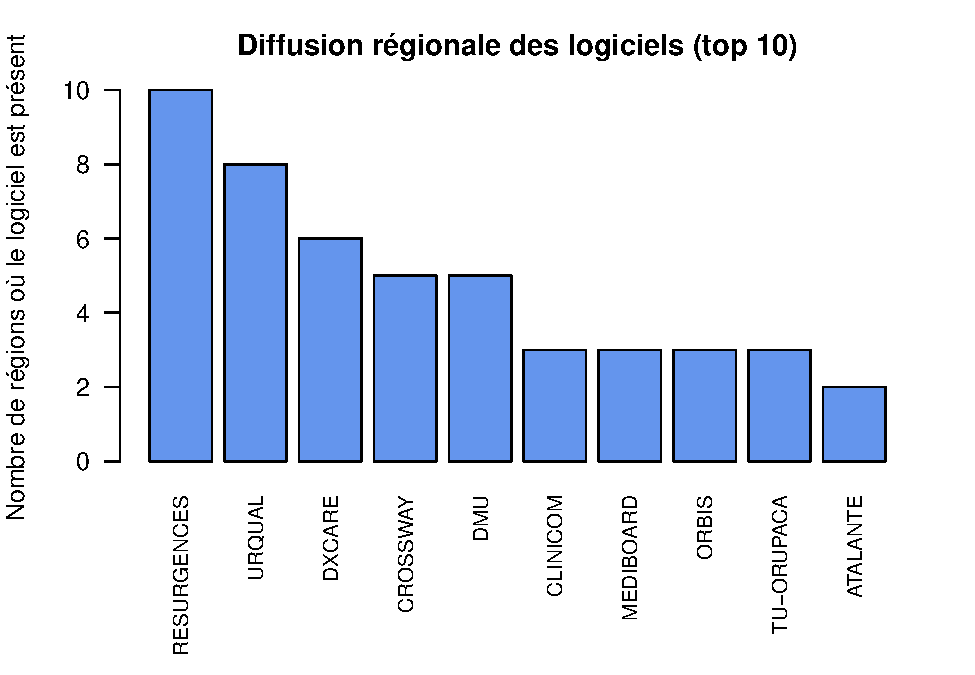
\includegraphics{septembre2015_files/figure-latex/unnamed-chunk-14-2.pdf}

\section{Analyse des RPU}\label{analyse-des-rpu}

Nombre de RPU produits: 2323895

\subsection{Nombre de RPU par
logiciel}\label{nombre-de-rpu-par-logiciel}

\begin{verbatim}
                      Nb de RPU
URQUAL                   377231
TU-ORUPACA               367714
RESURGENCES              347104
DMU                      299522
DXCARE                   135660
CROSSWAY                 106311
ATALANTE                  59400
DPU                       45087
SIDSU                     44401
MEDIBOARD                 42388
FIRSTNET                  33773
SILLAGE URGENCES          32519
CLINICOM                  27188
MÉDICAL OBJECT            25154
CORTEXTE                  24738
ORUV2                     21430
EXPERT SANTE              20440
POLYMEDIS                 20363
DOPASOIN                  18658
ANTARES                   17948
DEVELOPPEMENT INTERNE     17490
EXPERTIZ                  15215
DX CARE                   14920
EXAGONE                   14004
ORBIS                     13694
SILLAGE DMU               11801
TRACK CARE                11345
DOPA URGENCES             10420
RPUEXPRESS                10410
M-PLUS                     9970
H+ACUTE                    9762
SHAREGATE                  8639
CLIMCO                     8565
SIGEMS                     7231
SANOCOM                    7150
OSOFT                      7050
SPEC 4D                    7015
MEDIS                      6974
CORA URGENCE               6618
URGEST                     6321
MEDINTUX                   6224
MEDIWERE                   5676
NAFAMA                     5156
QCARE                      5131
AXIGATE                    4282
E SHERPA                   4090
OSIRIS                     4038
DIAMMS                     3666
CORPUS                     3601
EMED                       3246
MEDIBASE                   2913
HOPITAL MANAGER            2644
EQUAFILE                   1605
\end{verbatim}

\subsection{Nombre de jours manquants}\label{nombre-de-jours-manquants}

\subsubsection{Par logiciel}\label{par-logiciel}

\begin{verbatim}
                      Nb de jours manquants
DOPASOIN                             118.00
URQUAL                               117.00
EMED                                 100.00
TU-ORUPACA                            90.00
CROSSWAY                              63.03
ORBIS                                 55.00
SILLAGE URGENCES                      42.00
OSOFT                                 21.00
DMU                                   20.00
DEVELOPPEMENT INTERNE                 17.00
DPU                                    9.00
CLINICOM                               8.00
RESURGENCES                            5.56
MEDIBOARD                              4.00
HOPITAL MANAGER                        3.00
ANTARES                                2.00
ATALANTE                               2.00
E SHERPA                               2.00
EQUAFILE                               0.31
FIRSTNET                               0.04
AXIGATE                                0.00
CLIMCO                                 0.00
CORA URGENCE                           0.00
CORPUS                                 0.00
CORTEXTE                               0.00
DIAMMS                                 0.00
DOPA URGENCES                          0.00
DX CARE                                0.00
DXCARE                                 0.00
EXAGONE                                0.00
EXPERT SANTE                           0.00
EXPERTIZ                               0.00
H+ACUTE                                0.00
M-PLUS                                 0.00
MEDIBASE                               0.00
MÉDICAL OBJECT                         0.00
MEDINTUX                               0.00
MEDIS                                  0.00
MEDIWERE                               0.00
NAFAMA                                 0.00
ORUV2                                  0.00
OSIRIS                                 0.00
POLYMEDIS                              0.00
QCARE                                  0.00
RPUEXPRESS                             0.00
SANOCOM                                0.00
SHAREGATE                              0.00
SIDSU                                  0.00
SIGEMS                                 0.00
SILLAGE DMU                            0.00
SPEC 4D                                0.00
TRACK CARE                             0.00
URGEST                                 0.00
\end{verbatim}

\begin{verbatim}
                        Min   Max moyenne médiane ecart.type Nb   Q25   Q75
ANTARES                0.00  1.00  0.5000    0.50      0.577  4  0.00  1.00
ATALANTE               0.00  1.00  0.1538    0.00      0.376 13  0.00  0.00
AXIGATE                0.00  0.00  0.0000    0.00         NA  1  0.00  0.00
CLIMCO                 0.00  0.00  0.0000    0.00         NA  1  0.00  0.00
CLINICOM               0.00  4.00  1.6000    0.00      2.191  5  0.00  4.00
CORA URGENCE           0.00  0.00  0.0000    0.00         NA  1  0.00  0.00
CORPUS                  Inf  -Inf     NaN      NA         NA  1    NA    NA
CORTEXTE               0.00  0.00  0.0000    0.00      0.000  4  0.00  0.00
CROSSWAY               0.00 63.00  3.5017    0.00     14.849 20  0.00  0.00
DEVELOPPEMENT INTERNE  0.00 17.00  4.2500    0.00      8.500  4  0.00  4.25
DIAMMS                 0.00  0.00  0.0000    0.00      0.000  2  0.00  0.00
DMU                    0.00 16.00  0.4167    0.00      2.314 50  0.00  0.00
DOPA URGENCES          0.00  0.00  0.0000    0.00      0.000  3  0.00  0.00
DOPASOIN               0.00 59.00 19.6667    0.00     30.467  6  0.00 44.25
DPU                    0.00  9.00  2.2500    0.00      4.500  4  0.00  2.25
DX CARE                0.00  0.00  0.0000    0.00      0.000  2  0.00  0.00
DXCARE                 0.00  0.00  0.0000    0.00      0.000 18  0.00  0.00
E SHERPA               2.00  2.00  2.0000    2.00         NA  1  2.00  2.00
EMED                  50.00 50.00 50.0000   50.00      0.000  2 50.00 50.00
EQUAFILE               0.31  0.31  0.3100    0.31         NA  1  0.31  0.31
EXAGONE                0.00  0.00  0.0000    0.00      0.000  3  0.00  0.00
EXPERT SANTE           0.00  0.00  0.0000    0.00      0.000  3  0.00  0.00
EXPERTIZ               0.00  0.00  0.0000    0.00      0.000  3  0.00  0.00
FIRSTNET               0.00  0.04  0.0067    0.00      0.016  6  0.00  0.00
H+ACUTE                 Inf  -Inf     NaN      NA         NA  2    NA    NA
HOPITAL MANAGER        0.00  3.00  1.5000    1.50      2.121  2  0.75  2.25
M-PLUS                 0.00  0.00  0.0000    0.00         NA  1  0.00  0.00
MEDIBASE               0.00  0.00  0.0000    0.00         NA  1  0.00  0.00
MEDIBOARD              0.00  1.00  0.4444    0.00      0.527  9  0.00  1.00
MÉDICAL OBJECT         0.00  0.00  0.0000    0.00      0.000  4  0.00  0.00
MEDINTUX               0.00  0.00  0.0000    0.00         NA  1  0.00  0.00
MEDIS                  0.00  0.00  0.0000    0.00         NA  1  0.00  0.00
MEDIWERE               0.00  0.00  0.0000    0.00         NA  1  0.00  0.00
NAFAMA                 0.00  0.00  0.0000    0.00         NA  1  0.00  0.00
ORBIS                  0.00 25.00 13.7500   15.00     13.150  6  3.75 25.00
ORUV2                  0.00  0.00  0.0000    0.00      0.000  8  0.00  0.00
OSIRIS                 0.00  0.00  0.0000    0.00      0.000  2  0.00  0.00
OSOFT                  0.00 21.00 10.5000   10.50     14.849  2  5.25 15.75
POLYMEDIS              0.00  0.00  0.0000    0.00      0.000  5  0.00  0.00
QCARE                  0.00  0.00  0.0000    0.00         NA  1  0.00  0.00
RESURGENCES            0.00  5.00  0.1853    0.00      0.911 47  0.00  0.00
RPUEXPRESS             0.00  0.00  0.0000    0.00      0.000  4  0.00  0.00
SANOCOM                0.00  0.00  0.0000    0.00      0.000  2  0.00  0.00
SHAREGATE              0.00  0.00  0.0000    0.00      0.000  2  0.00  0.00
SIDSU                  0.00  0.00  0.0000    0.00      0.000  9  0.00  0.00
SIGEMS                 0.00  0.00  0.0000    0.00      0.000  3  0.00  0.00
SILLAGE DMU            0.00  0.00  0.0000    0.00      0.000  2  0.00  0.00
SILLAGE URGENCES       0.00 42.00  5.2500    0.00     14.849  8  0.00  0.00
SPEC 4D                0.00  0.00  0.0000    0.00         NA  1  0.00  0.00
TRACK CARE             0.00  0.00  0.0000    0.00         NA  1  0.00  0.00
TU-ORUPACA             0.00 90.00  1.9149    0.00     13.128 47  0.00  0.00
URGEST                 0.00  0.00  0.0000    0.00         NA  1  0.00  0.00
URQUAL                 0.00 85.00  3.0000    0.00     13.792 40  0.00  0.50
\end{verbatim}

\subsubsection{Par région}\label{par-region}

\begin{verbatim}
                   Nb de jours manquants
MIDI PYRENEES                     222.00
PACA                              180.00
RHONE ALPES                        73.00
ALSACE                             64.00
AQUITAINE                          63.00
BRETAGNE                           52.00
BOURGOGNE                          21.00
CHAMPAGNE ARDENNES                  3.00
FRANCHE COMTE                       0.94
LIMOUSIN                            0.00
LORRAINE                            0.00
\end{verbatim}

\section{Indicateurs}\label{indicateurs}

Trois indicateurs ont été retenus:

\begin{itemize}
\tightlist
\item
  Date de naissance
\item
  Diagnostic principal (DP)
\item
  Mode de sortie
\end{itemize}

Chaque indicateur a été évalué sur deux critères: \textbf{conformité} et
\textbf{exhaustivité}.

\subsection{Date de naissance}\label{date-de-naissance}

\begin{itemize}
\tightlist
\item
  taux de conformité:
\end{itemize}

\begin{verbatim}
   Min. 1st Qu.  Median    Mean 3rd Qu.    Max.    NA's 
      0     100     100     100     100     100       7 
\end{verbatim}

\begin{itemize}
\tightlist
\item
  conformité par outil:
\end{itemize}

\begin{verbatim}
                      Min Max moyenne médiane ecart.type Nb Q25 Q75
ANTARES               100 100     100     100     0.0000  4 100 100
ATALANTE              100 100     100     100     0.0000 13 100 100
AXIGATE               100 100     100     100         NA  1 100 100
CLIMCO                100 100     100     100         NA  1 100 100
CLINICOM              100 100     100     100     0.0000  5 100 100
CORA URGENCE          100 100     100     100         NA  1 100 100
CORPUS                100 100     100     100         NA  1 100 100
CORTEXTE              100 100     100     100     0.0000  4 100 100
CROSSWAY              100 100     100     100     0.0067 20 100 100
DEVELOPPEMENT INTERNE 100 100     100     100     0.0346  4 100 100
DIAMMS                100 100     100     100     0.0000  2 100 100
DMU                   100 100     100     100     0.0000 50 100 100
DOPA URGENCES         100 100     100     100     0.0000  3 100 100
DOPASOIN              100 100     100     100     0.0207  6 100 100
DPU                   100 100     100     100     0.0000  4 100 100
DX CARE               100 100     100     100     0.0000  2 100 100
DXCARE                100 100     100     100     0.0000 18 100 100
E SHERPA              100 100     100     100         NA  1 100 100
EMED                  100 100     100     100     0.0000  2 100 100
EQUAFILE              100 100     100     100         NA  1 100 100
EXAGONE               100 100     100     100     0.0000  3 100 100
EXPERT SANTE          100 100     100     100     0.0000  3 100 100
EXPERTIZ              100 100     100     100     0.0000  3 100 100
FIRSTNET              100 100     100     100     0.0000  6 100 100
H+ACUTE               100 100     100     100     0.0000  2 100 100
HOPITAL MANAGER       100 100     100     100     0.0000  2 100 100
M-PLUS                100 100     100     100         NA  1 100 100
MEDIBASE              100 100     100     100         NA  1 100 100
MEDIBOARD             100 100     100     100     0.0088  9 100 100
MÉDICAL OBJECT        100 100     100     100     0.0000  4 100 100
MEDINTUX              100 100     100     100         NA  1 100 100
MEDIS                 100 100     100     100         NA  1 100 100
MEDIWERE              100 100     100     100         NA  1 100 100
NAFAMA                100 100     100     100         NA  1 100 100
ORBIS                 100 100     100     100     0.0000  6 100 100
ORUV2                  99 100     100     100     0.5621  8 100 100
OSIRIS                100 100     100     100     0.0000  2 100 100
OSOFT                 100 100     100     100     0.0000  2 100 100
POLYMEDIS             100 100     100     100     0.0000  5 100 100
QCARE                 100 100     100     100         NA  1 100 100
RESURGENCES           100 100     100     100     0.0074 47 100 100
RPUEXPRESS            100 100     100     100     0.0635  4 100 100
SANOCOM               100 100     100     100     0.0000  2 100 100
SHAREGATE             100 100     100     100     0.0000  2 100 100
SIDSU                 100 100     100     100     0.0000  9 100 100
SIGEMS                100 100     100     100     0.0000  3 100 100
SILLAGE DMU           100 100     100     100     0.0000  2 100 100
SILLAGE URGENCES      100 100     100     100     0.0000  8 100 100
SPEC 4D               100 100     100     100         NA  1 100 100
TRACK CARE            100 100     100     100         NA  1 100 100
TU-ORUPACA              0 100      98     100    14.5865 47 100 100
URGEST                100 100     100     100         NA  1 100 100
URQUAL                100 100     100     100     0.0323 40 100 100
\end{verbatim}

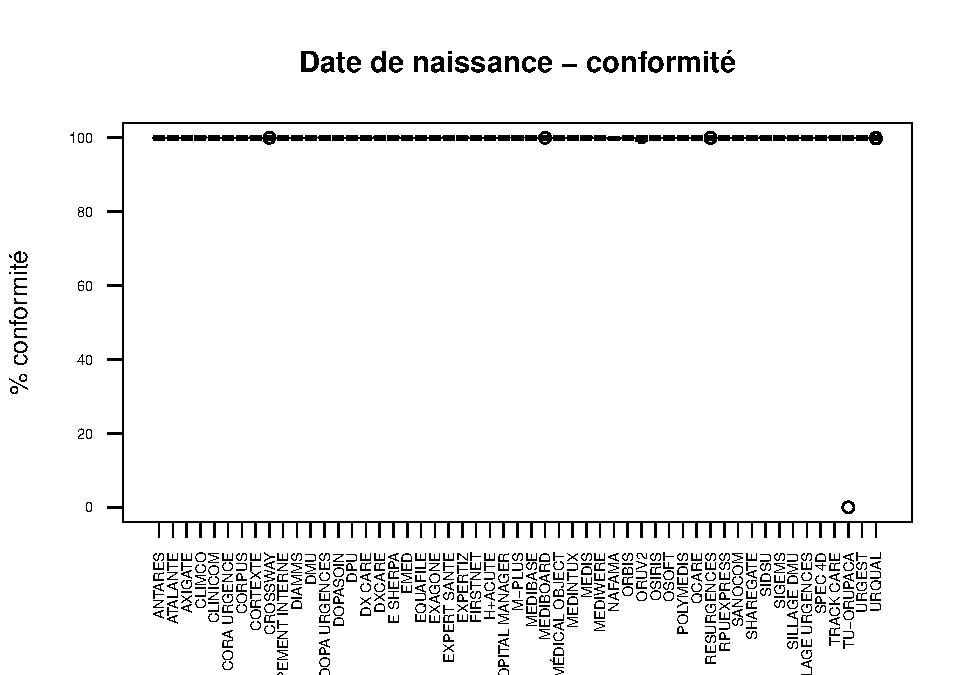
\includegraphics{septembre2015_files/figure-latex/unnamed-chunk-20-1.pdf}

\begin{itemize}
\tightlist
\item
  taux d'exhaustivité:
\end{itemize}

\begin{verbatim}
   Min. 1st Qu.  Median    Mean 3rd Qu.    Max.    NA's 
      0     100     100     100     100     100      20 
\end{verbatim}

\begin{itemize}
\tightlist
\item
  exhaustivité par outil
  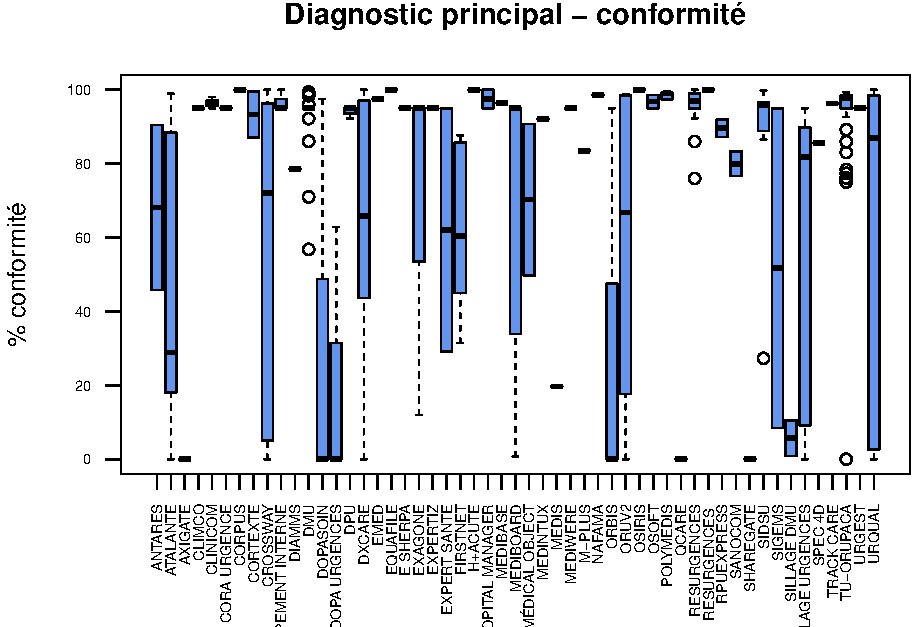
\includegraphics{septembre2015_files/figure-latex/unnamed-chunk-22-1.pdf}
\end{itemize}

\subsection{Diagnostic (DP)}\label{diagnostic-dp}

\subsubsection{taux de conformité:}\label{taux-de-conformite}

\begin{verbatim}
   Min. 1st Qu.  Median    Mean 3rd Qu.    Max.    NA's 
      0      85      95      80      99     100       8 
\end{verbatim}

\begin{itemize}
\tightlist
\item
  \% de DP conformes: 97.85
\end{itemize}

\subsubsection{conformité par outil}\label{conformite-par-outil}

\begin{verbatim}
                         Min   Max moyenne médiane ecart.type Nb     Q25     Q75
ANTARES               100.00 100.0  100.00  100.00      0.000  4 100.000 100.000
ATALANTE                0.00 100.0   92.15  100.00     27.694 13 100.000 100.000
AXIGATE                 0.00   0.0    0.00    0.00         NA  1   0.000   0.000
CLIMCO                 95.00  95.0   95.00   95.00         NA  1  95.000  95.000
CLINICOM               95.00 100.0   98.21   98.03      2.048  5  98.030 100.000
CORA URGENCE           95.00  95.0   95.00   95.00         NA  1  95.000  95.000
CORPUS                100.00 100.0  100.00  100.00         NA  1 100.000 100.000
CORTEXTE               87.11  99.5   93.30   93.30      7.148  4  87.110  99.490
CROSSWAY                0.00 100.0   62.50   79.27     40.163 20  29.955  98.140
DEVELOPPEMENT INTERNE  95.00 100.0   97.50   97.50      2.887  4  95.000 100.000
DIAMMS                 78.56  78.6   78.56   78.56      0.000  2  78.560  78.560
DMU                    56.80 100.0   94.28   95.00      6.838 50  95.000  95.000
DOPA URGENCES           0.00  62.9   20.97    0.00     36.315  3   0.000  31.450
DOPASOIN                0.00  97.5   32.50    0.00     50.344  6   0.000  73.117
DPU                    92.18  95.0   93.59   93.59      1.628  4  92.180  95.000
DX CARE               100.00 100.0  100.00  100.00      0.000  2 100.000 100.000
DXCARE                  0.00 100.0   71.93   96.66     38.161 18  55.900 100.000
E SHERPA               95.00  95.0   95.00   95.00         NA  1  95.000  95.000
EMED                   97.54  97.5   97.54   97.54      0.000  2  97.540  97.540
EQUAFILE              100.00 100.0  100.00  100.00         NA  1 100.000 100.000
EXAGONE                12.00  95.0   67.33   95.00     47.920  3  53.500  95.000
EXPERT SANTE           29.20  95.0   51.13   29.20     37.990  3  29.200  62.100
EXPERTIZ               95.00  95.0   95.00   95.00      0.000  3  95.000  95.000
FIRSTNET               31.40  87.7   61.77   60.40     22.257  6  47.975  80.250
H+ACUTE               100.00 100.0  100.00  100.00      0.000  2 100.000 100.000
HOPITAL MANAGER        95.00 100.0   97.50   97.50      3.536  2  96.250  98.750
M-PLUS                 83.50  83.5   83.50   83.50         NA  1  83.500  83.500
MEDIBASE               96.40  96.4   96.40   96.40         NA  1  96.400  96.400
MEDIBOARD               0.73  95.0   52.62   43.20     42.193  9  24.480  95.000
MÉDICAL OBJECT         49.76  90.8   70.27   70.27     23.677  4  49.760  90.770
MEDINTUX               92.15  92.2   92.15   92.15         NA  1  92.150  92.150
MEDIS                  19.70  19.7   19.70   19.70         NA  1  19.700  19.700
MEDIWERE               95.00  95.0   95.00   95.00         NA  1  95.000  95.000
NAFAMA                 98.50  98.5   98.50   98.50         NA  1  98.500  98.500
ORBIS                   0.00 100.0   73.75   97.50     49.223  6  71.250 100.000
ORUV2                   0.00  98.9   58.10   66.75     45.222  8  26.543  98.315
OSIRIS                100.00 100.0  100.00  100.00      0.000  2 100.000 100.000
OSOFT                  95.00  98.6   96.80   96.80      2.546  2  95.900  97.700
POLYMEDIS              97.40  99.7   98.50   99.00      1.044  5  97.400  99.000
QCARE                   0.00   0.0    0.00    0.00         NA  1   0.000   0.000
RESURGENCES            86.00 100.0   97.92   99.50      2.967 47  96.850 100.000
RPUEXPRESS             87.22  92.0   89.59   89.59      2.731  4  87.220  91.950
SANOCOM                76.70  83.3   80.00   80.00      4.667  2  78.350  81.650
SHAREGATE               0.00   0.1    0.05    0.05      0.071  2   0.025   0.075
SIDSU                  27.30  99.8   87.06   95.80     22.825  9  88.800  96.700
SIGEMS                  8.40  95.0   51.70   51.70     61.235  3  30.050  73.350
SILLAGE DMU             0.90  10.5    5.70    5.70      6.788  2   3.300   8.100
SILLAGE URGENCES        0.00  95.0   57.06   81.80     42.869  8  13.750  88.975
SPEC 4D                85.57  85.6   85.57   85.57         NA  1  85.570  85.570
TRACK CARE             96.30  96.3   96.30   96.30         NA  1  96.300  96.300
TU-ORUPACA              0.00  99.3   93.02   97.62     15.317 47  95.325  98.405
URGEST                 95.00  95.0   95.00   95.00         NA  1  95.000  95.000
URQUAL                  0.00 100.0   62.91   91.20     42.733 40   5.840  98.505
\end{verbatim}

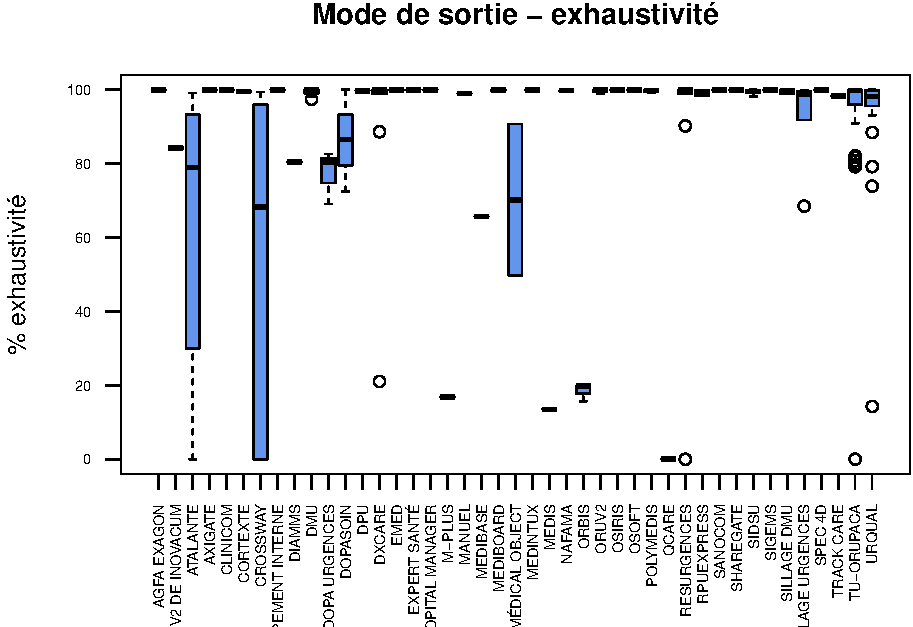
\includegraphics{septembre2015_files/figure-latex/unnamed-chunk-24-1.pdf}

\begin{itemize}
\tightlist
\item
  taux de exhaustivité:
\end{itemize}

\begin{verbatim}
   Min. 1st Qu.  Median    Mean 3rd Qu.    Max.    NA's 
      0      59      94      74      99     100       8 
\end{verbatim}

\begin{itemize}
\tightlist
\item
  exhaustivité par outil
\end{itemize}

\begin{verbatim}
                        Min   Max moyenne médiane ecart.type Nb     Q25     Q75
ANTARES                45.8  90.5   68.18   68.18     25.790  4  45.840  90.510
ATALANTE                0.0  99.0   44.52   39.80     37.426 13  18.040  88.480
AXIGATE                 0.0   0.0    0.00    0.00         NA  1   0.000   0.000
CLIMCO                 38.0  38.0   38.00   38.00         NA  1  38.000  38.000
CLINICOM               72.0  98.0   92.07   96.14     11.258  5  96.140  98.030
CORA URGENCE           95.0  95.0   95.00   95.00         NA  1  95.000  95.000
CORPUS                100.0 100.0  100.00  100.00         NA  1 100.000 100.000
CORTEXTE               87.6  99.5   93.54   93.54      6.899  4  87.570  99.520
CROSSWAY                0.0 100.0   63.97   79.27     38.407 20  31.950  98.090
DEVELOPPEMENT INTERNE  83.0 100.0   94.50   97.50      8.021  4  92.000 100.000
DIAMMS                 78.7  78.7   78.72   78.72      0.000  2  78.720  78.720
DMU                     2.0 100.0   89.01   95.00     16.799 50  86.080  97.500
DOPA URGENCES           0.0  62.9   20.97    0.00     36.315  3   0.000  31.450
DOPASOIN                0.0  97.7   32.57    0.00     50.457  6   0.000  73.282
DPU                    87.0  97.0   92.09   92.18      4.084  4  90.885  93.385
DX CARE                 9.1   9.1    9.10    9.10      0.000  2   9.100   9.100
DXCARE                  0.0  98.9   60.77   59.20     34.641 18  52.240  95.000
E SHERPA                0.0   0.0    0.00    0.00         NA  1   0.000   0.000
EMED                   97.6  97.6   97.60   97.60      0.000  2  97.600  97.600
EQUAFILE              100.0 100.0  100.00  100.00         NA  1 100.000 100.000
EXAGONE                 0.0  12.0    5.33    4.00      6.110  3   2.000   8.000
EXPERT SANTE           29.2  95.0   51.15   29.22     37.978  3  29.220  62.110
EXPERTIZ               82.0  94.0   88.67   90.00      6.110  3  86.000  92.000
FIRSTNET              100.0 100.0  100.00  100.00      0.000  6 100.000 100.000
H+ACUTE                99.0 100.0   99.50   99.50      0.707  2  99.250  99.750
HOPITAL MANAGER        95.0 100.0   97.50   97.50      3.536  2  96.250  98.750
M-PLUS                 83.5  83.5   83.50   83.50         NA  1  83.500  83.500
MEDIBASE               96.4  96.4   96.40   96.40         NA  1  96.400  96.400
MEDIBOARD               0.0  43.2   10.85    1.00     15.878  9   0.730  24.480
MÉDICAL OBJECT         49.8  90.8   70.27   70.27     23.677  4  49.760  90.770
MEDINTUX              100.0 100.0  100.00  100.00         NA  1 100.000 100.000
MEDIS                  19.7  19.7   19.70   19.70         NA  1  19.700  19.700
MEDIWERE              100.0 100.0  100.00  100.00         NA  1 100.000 100.000
NAFAMA                 99.8  99.8   99.80   99.80         NA  1  99.800  99.800
ORBIS                   0.0   0.0    0.00    0.00      0.000  6   0.000   0.000
ORUV2                   0.0  98.9   58.19   66.92     45.306  8  26.543  98.562
OSIRIS                100.0 100.0  100.00  100.00      0.000  2 100.000 100.000
OSOFT                   0.0  98.6   49.30   49.30     69.721  2  24.650  73.950
POLYMEDIS              97.4  99.7   98.74   99.00      0.847  5  98.600  99.000
QCARE                   0.0   0.0    0.00    0.00         NA  1   0.000   0.000
RESURGENCES            76.0 100.0   97.19   99.00      5.316 47  97.410 100.000
RPUEXPRESS             87.2  92.0   89.59   89.59      2.731  4  87.220  91.950
SANOCOM                76.7  83.3   80.00   80.00      4.667  2  78.350  81.650
SHAREGATE               0.0   0.1    0.05    0.05      0.071  2   0.025   0.075
SIDSU                  27.3  99.8   87.06   95.80     22.825  9  88.800  96.700
SIGEMS                  8.4  80.0   44.20   44.20     50.629  3  26.300  62.100
SILLAGE DMU             0.9  10.5    5.70    5.70      6.788  2   3.300   8.100
SILLAGE URGENCES        0.0  95.0   57.06   81.80     42.869  8  13.750  88.975
SPEC 4D                85.6  85.6   85.57   85.57         NA  1  85.570  85.570
TRACK CARE             96.3  96.3   96.30   96.30         NA  1  96.300  96.300
TU-ORUPACA              0.0  99.3   93.04   97.62     15.320 47  95.420  98.405
URGEST                 98.0  98.0   98.00   98.00         NA  1  98.000  98.000
URQUAL                  0.0 100.0   61.18   86.00     42.678 40   5.840  98.655
\end{verbatim}

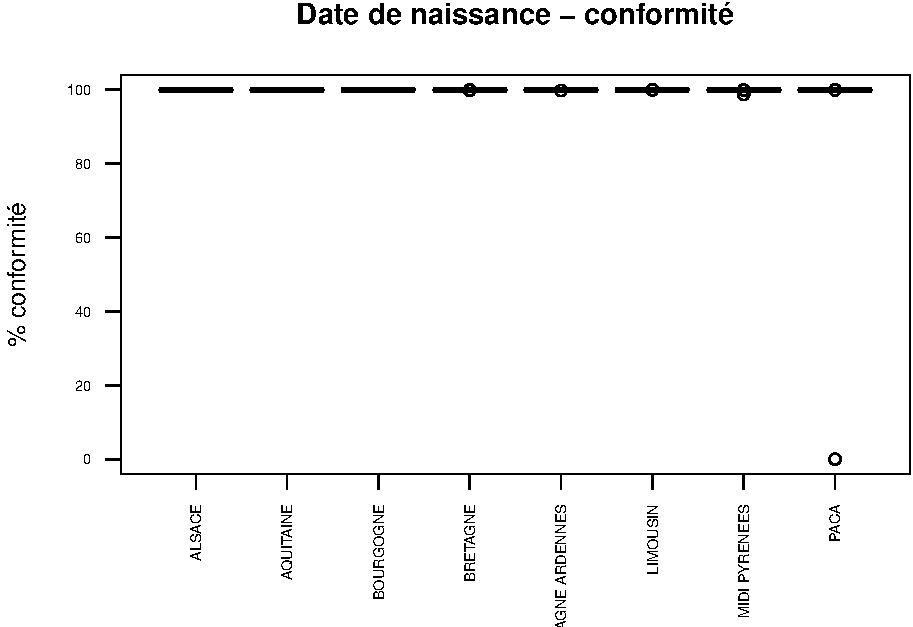
\includegraphics{septembre2015_files/figure-latex/unnamed-chunk-26-1.pdf}

\subsubsection{correlation
exhaustivité-conformité}\label{correlation-exhaustivite-conformite}

\begin{Shaded}
\begin{Highlighting}[]
\CommentTok{# on ne garde que les couples complets}
\NormalTok{ok <-}\StringTok{ }\NormalTok{d[}\KeywordTok{which}\NormalTok{(}\KeywordTok{complete.cases}\NormalTok{(d$DP_exhaus, d$DP_confor)),]}
\KeywordTok{cor}\NormalTok{(ok$DP_exhaus, ok$DP_confor)}
\end{Highlighting}
\end{Shaded}

\begin{verbatim}
[1] 0.72
\end{verbatim}

\begin{Shaded}
\begin{Highlighting}[]
\KeywordTok{plot}\NormalTok{(ok$DP_exhaus, ok$DP_confor)}
\end{Highlighting}
\end{Shaded}

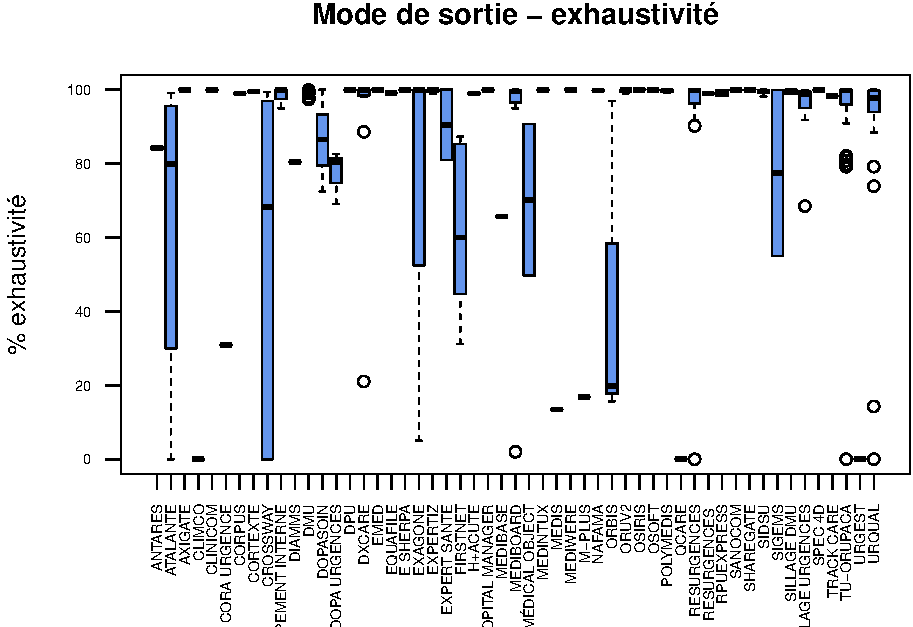
\includegraphics{septembre2015_files/figure-latex/unnamed-chunk-27-1.pdf}

\subsection{Mode de sortie (MS)}\label{mode-de-sortie-ms}

\begin{itemize}
\tightlist
\item
  taux de conformité:
\end{itemize}

\begin{verbatim}
   Min. 1st Qu.  Median    Mean 3rd Qu.    Max.    NA's 
      1      15      44      50      82     113      70 
\end{verbatim}

\begin{itemize}
\tightlist
\item
  conformité par outil
\end{itemize}

\begin{verbatim}
                      Min  Max moyenne médiane ecart.type Nb Q25 Q75
ANTARES                15   15    15.0      15       0.00  4  15  15
ATALANTE                2   75    18.6      15      17.32 13  15  15
AXIGATE               104  104   104.0     104         NA  1 104 104
CLIMCO                Inf -Inf     NaN      NA         NA  1  NA  NA
CLINICOM               15   69    42.0      42      31.18  5  15  69
CORA URGENCE          Inf -Inf     NaN      NA         NA  1  NA  NA
CORPUS                 75   75    75.0      75         NA  1  75  75
CORTEXTE               84   92    88.0      88       4.62  4  84  92
CROSSWAY                1   85    35.5      30      31.49 20   4  62
DEVELOPPEMENT INTERNE 103  103   103.0     103       0.00  4 103 103
DIAMMS                 33   33    33.0      33       0.00  2  33  33
DMU                    13  109    37.7      15      35.00 50  13  62
DOPA URGENCES          25   37    31.3      32       6.03  3  28  34
DOPASOIN               26   39    31.0      28       6.26  6  26  36
DPU                    95   95    95.0      95       0.00  4  95  95
DX CARE                15   15    15.0      15       0.00  2  15  15
DXCARE                 13  104    40.8      15      35.70 18  14  67
E SHERPA              Inf -Inf     NaN      NA         NA  1  NA  NA
EMED                   15   15    15.0      15       0.00  2  15  15
EQUAFILE               11   11    11.0      11         NA  1  11  11
EXAGONE                13   13    13.0      13         NA  3  13  13
EXPERT SANTE          108  108   108.0     108       0.00  3 108 108
EXPERTIZ              Inf -Inf     NaN      NA         NA  3  NA  NA
FIRSTNET                4    6     4.3       4       0.82  6   4   4
H+ACUTE                75   75    75.0      75       0.00  2  75  75
HOPITAL MANAGER        13   13    13.0      13       0.00  2  13  13
M-PLUS                 18   18    18.0      18         NA  1  18  18
MEDIBASE               22   22    22.0      22         NA  1  22  22
MEDIBOARD              87  110   100.4     109      12.24  9  87 109
MÉDICAL OBJECT         21   41    31.0      31      11.55  4  21  41
MEDINTUX               15   15    15.0      15         NA  1  15  15
MEDIS                  16   16    16.0      16         NA  1  16  16
MEDIWERE              Inf -Inf     NaN      NA         NA  1  NA  NA
NAFAMA                 96   96    96.0      96         NA  1  96  96
ORBIS                  15   19    16.3      15       2.31  6  15  17
ORUV2                  20  107    68.5      74      33.42  8  58  84
OSIRIS                 15   15    15.0      15       0.00  2  15  15
OSOFT                  14   14    14.0      14         NA  2  14  14
POLYMEDIS              81  104    94.2      96      10.45  5  86 104
QCARE                   4    4     4.0       4         NA  1   4   4
RESURGENCES             3  112    43.1      15      34.22 47  14  75
RPUEXPRESS             45   47    46.0      46       1.15  4  45  47
SANOCOM                14   14    14.0      14       0.00  2  14  14
SHAREGATE              14   14    14.0      14       0.00  2  14  14
SIDSU                  14  104    68.4      80      32.61  9  64  86
SIGEMS                  1  104    52.5      52      72.83  3  27  78
SILLAGE DMU            14   72    43.0      43      41.01  2  28  58
SILLAGE URGENCES       24  104    68.9      72      25.50  8  60  84
SPEC 4D               111  111   111.0     111         NA  1 111 111
TRACK CARE             65   65    65.0      65         NA  1  65  65
TU-ORUPACA              4  113    73.7      87      35.17 47  44 105
URGEST                Inf -Inf     NaN      NA         NA  1  NA  NA
URQUAL                 13  101    50.6      52      31.40 40  15  80
\end{verbatim}

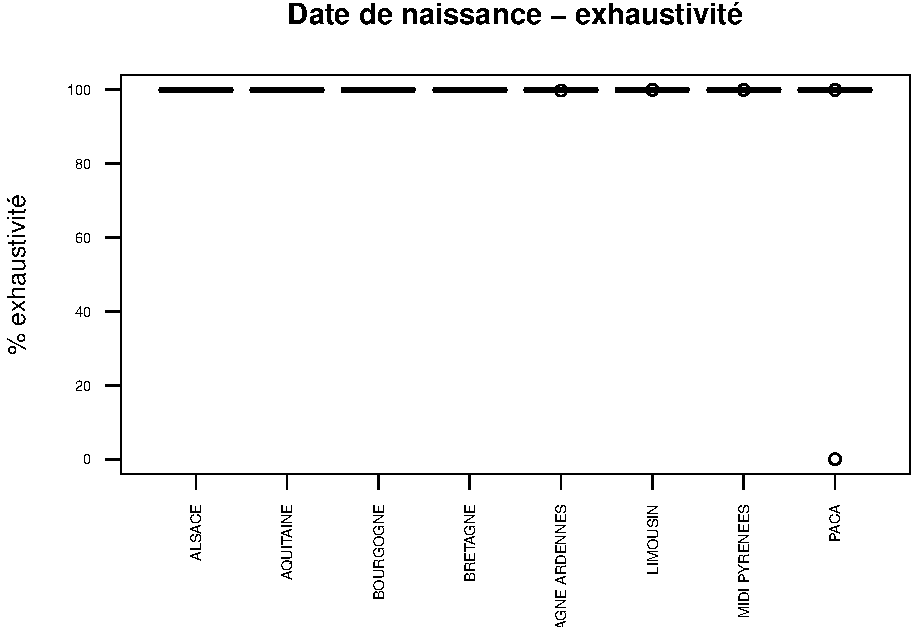
\includegraphics{septembre2015_files/figure-latex/unnamed-chunk-29-1.pdf}
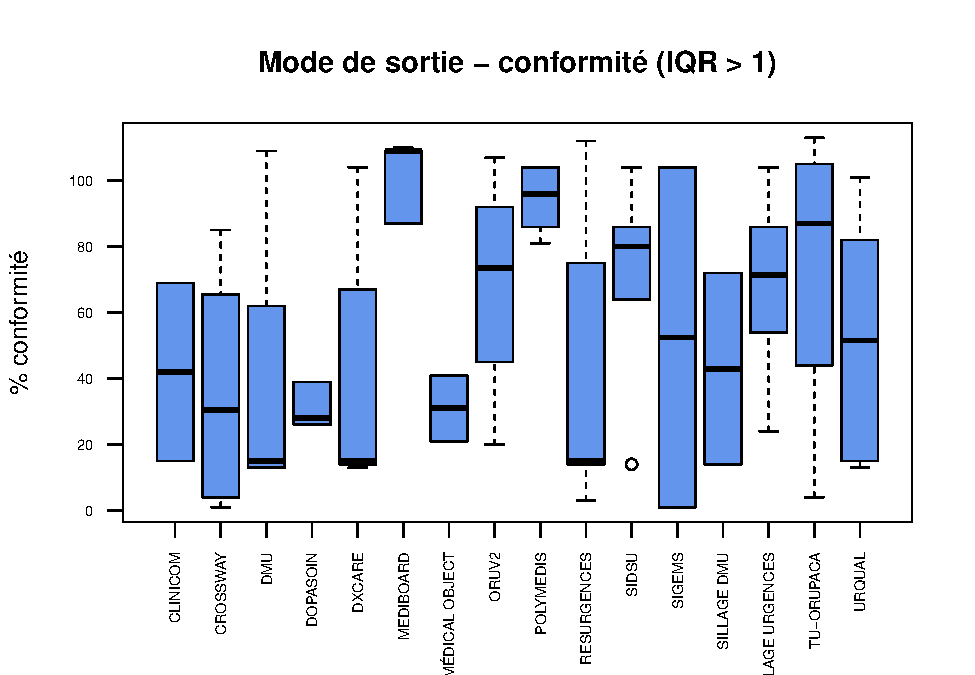
\includegraphics{septembre2015_files/figure-latex/unnamed-chunk-29-2.pdf}

\begin{itemize}
\tightlist
\item
  taux de exhaustivité:
\end{itemize}

\begin{verbatim}
   Min. 1st Qu.  Median    Mean 3rd Qu.    Max.    NA's 
      0      95      99      88     100     100       8 
\end{verbatim}

\begin{itemize}
\tightlist
\item
  exhaustivité par outil
\end{itemize}

\begin{verbatim}
               Min Max moyenne médiane ecart.type Nb   Q25 Q75 iqr
CROSSWAY         0  99      58      86         46 20  0.75  98  97
ATALANTE         0  99      70      81         35 13 30.03  96  66
EXAGONE          5 100      68     100         55  3 52.50 100  48
MÉDICAL OBJECT  50  91      70      70         24  4 49.76  91  41
FIRSTNET        31  87      61      60         22  6 47.68  80  32
ORBIS           16  97      37      18         40  6 15.70  39  23
SIGEMS          55 100      77      77         32  3 66.22  89  22
DOPASOIN        72 100      86      87         12  6 76.00  97  21
\end{verbatim}

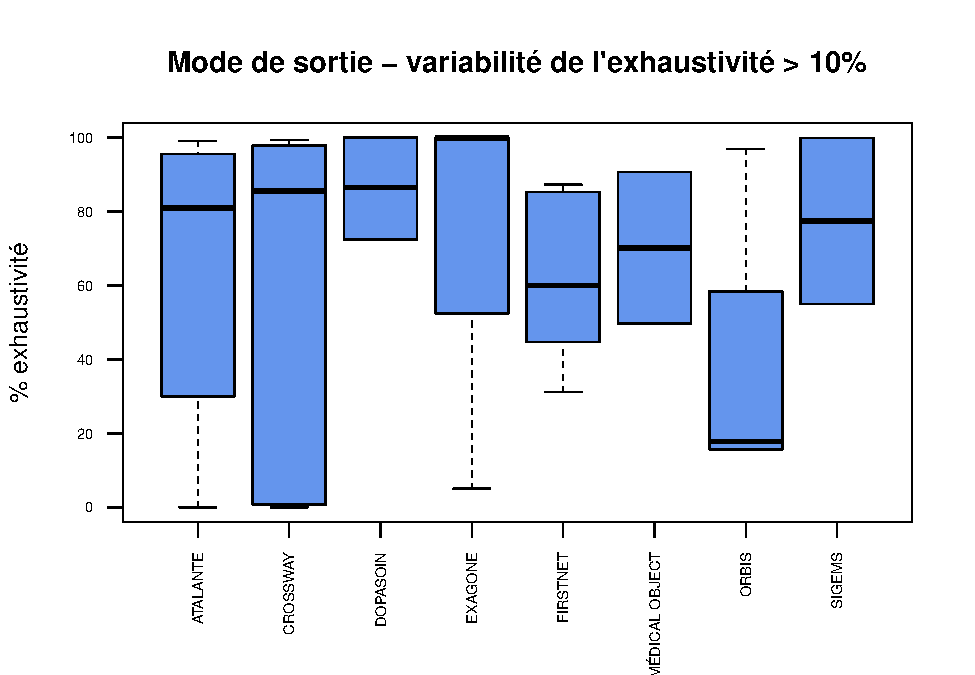
\includegraphics{septembre2015_files/figure-latex/unnamed-chunk-31-1.pdf}
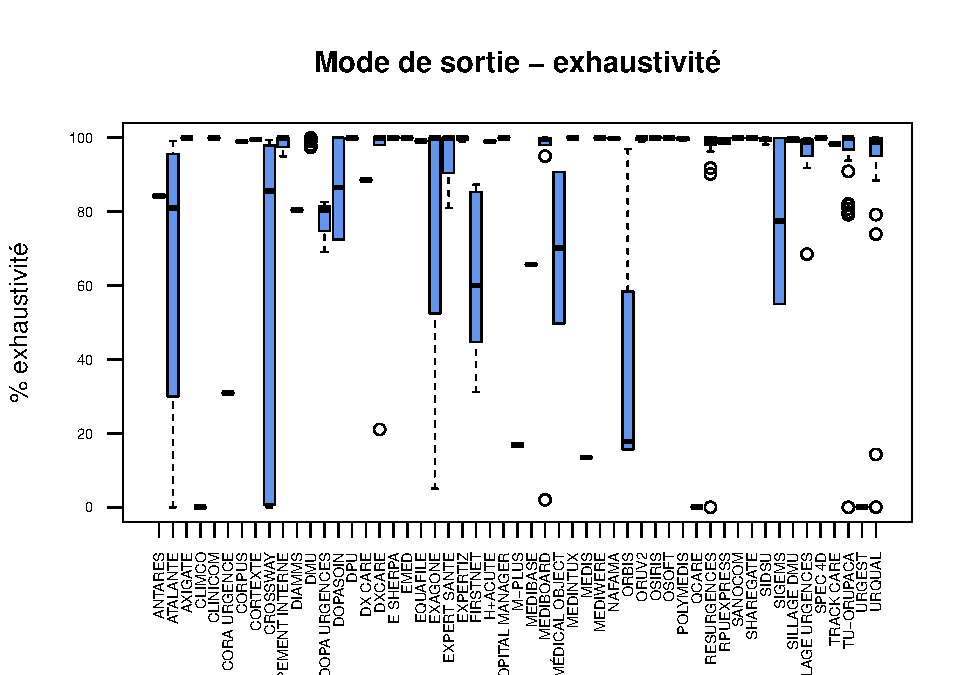
\includegraphics{septembre2015_files/figure-latex/unnamed-chunk-31-2.pdf}

\section{Conformité par région}\label{conformite-par-region}

\subsection{Date de naissance}\label{date-de-naissance-1}

\begin{verbatim}
                   Min Max moyenne médiane ecart.type Nb Q25 Q75
ALSACE             100 100     100     100      0.000 29 100 100
AQUITAINE          100 100     100     100      0.000 35 100 100
BOURGOGNE          100 100     100     100      0.000 23 100 100
BRETAGNE           100 100     100     100      0.037 30 100 100
CHAMPAGNE ARDENNES 100 100     100     100      0.050 16 100 100
FRANCHE COMTE      100 100     100     100      0.000 13 100 100
LIMOUSIN           100 100     100     100      0.017  9 100 100
LORRAINE           100 100     100     100      0.000 23 100 100
MIDI PYRENEES       99 100     100     100      0.206 74 100 100
PACA                 0 100      98     100     14.142 50 100 100
RHONE ALPES        100 100     100     100      0.000 70 100 100
\end{verbatim}

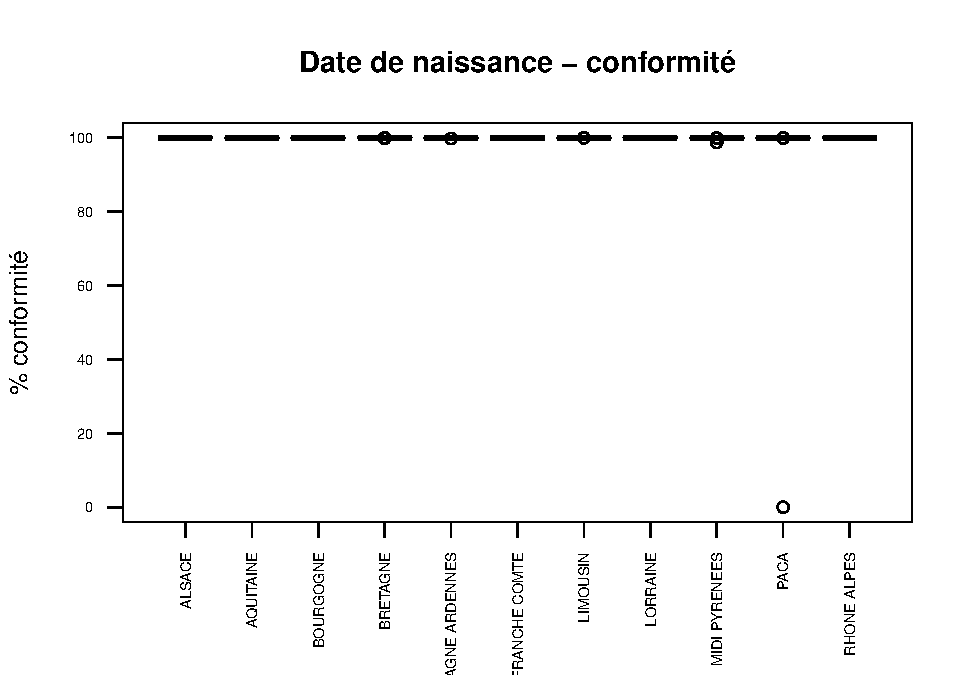
\includegraphics{septembre2015_files/figure-latex/unnamed-chunk-32-1.pdf}

\subsection{Diagnostic (DP)}\label{diagnostic-dp-1}

\begin{verbatim}
                   Min Max moyenne médiane ecart.type Nb   Q25 Q75
ALSACE             100 100     100     100        0.0 29 100.0 100
AQUITAINE            0 100      63      84       39.8 35  27.3  96
BOURGOGNE            0 100      62      95       45.0 23   3.8  99
BRETAGNE             0 100      64      91       41.0 30  18.7  98
CHAMPAGNE ARDENNES   0 100      68      92       41.1 16  44.9  99
FRANCHE COMTE        5 100      73      88       30.6 13  56.9  97
LIMOUSIN            86  99      97      98        4.3  9  97.6  99
LORRAINE           100 100     100     100        0.0 23 100.0 100
MIDI PYRENEES        0 100      70      92       37.7 74  35.4  98
PACA                 0  99      89      98       23.6 50  92.3  98
RHONE ALPES         95  95      95      95        0.0 70  95.0  95
\end{verbatim}

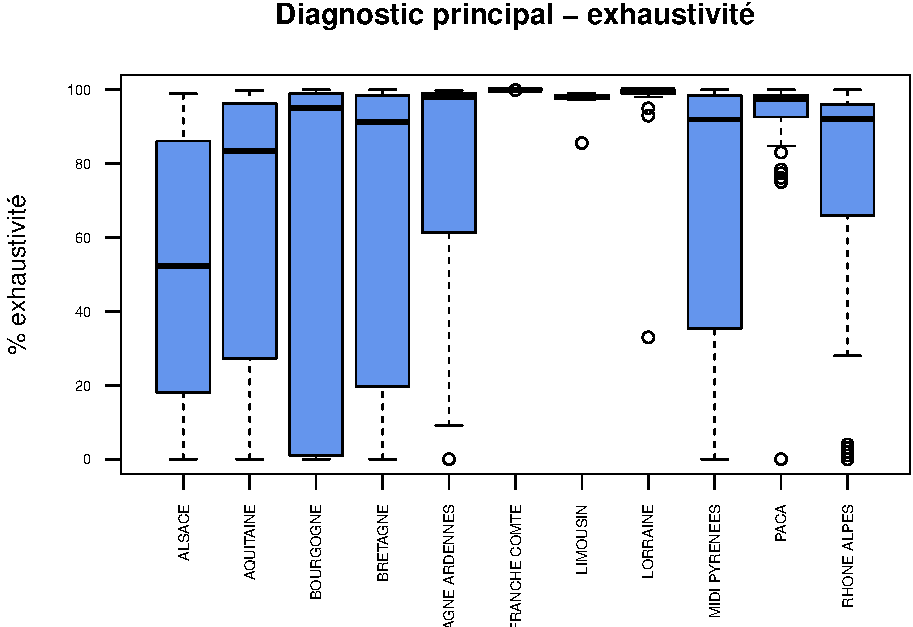
\includegraphics{septembre2015_files/figure-latex/unnamed-chunk-33-1.pdf}

\subsection{Mode de sortie (MS)}\label{mode-de-sortie-ms-1}

\begin{verbatim}
                   Min  Max moyenne médiane ecart.type Nb Q25 Q75
ALSACE              15   15    15.0      15        0.0 29  15  15
AQUITAINE            1  104    46.9      37       37.4 35  14  83
BOURGOGNE            2   79    27.2      13       27.1 23  13  54
BRETAGNE            14  110    49.8      54       33.0 30  14  74
CHAMPAGNE ARDENNES  14  104    62.3      68       36.3 16  29  96
FRANCHE COMTE        4   11     6.2       5        2.6 13   4   8
LIMOUSIN            15  112    52.2      15       45.1  9  15  90
LORRAINE            62   75    74.4      75        2.7 23  75  75
MIDI PYRENEES        4  111    55.7      47       35.0 74  21  87
PACA                 4  113    68.1      81       37.5 50  35 103
RHONE ALPES        Inf -Inf     NaN      NA         NA 70  NA  NA
\end{verbatim}

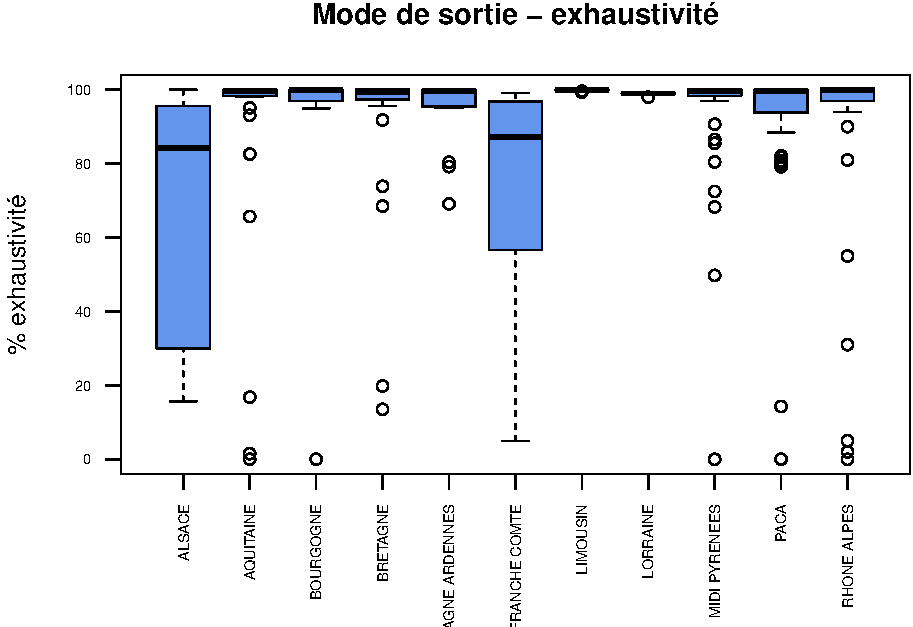
\includegraphics{septembre2015_files/figure-latex/unnamed-chunk-34-1.pdf}

\section{Exhaustivié et conformité par
région}\label{exhaustivie-et-conformite-par-region}

\subsection{Date de naissance}\label{date-de-naissance-2}

\begin{verbatim}
                   Min  Max moyenne médiane ecart.type Nb Q25 Q75
ALSACE             100  100     100     100      0.000 29 100 100
AQUITAINE          100  100     100     100      0.000 35 100 100
BOURGOGNE          100  100     100     100      0.000 23 100 100
BRETAGNE           100  100     100     100      0.000 30 100 100
CHAMPAGNE ARDENNES 100  100     100     100      0.050 16 100 100
FRANCHE COMTE      Inf -Inf     NaN      NA         NA 13  NA  NA
LIMOUSIN           100  100     100     100      0.017  9 100 100
LORRAINE           100  100     100     100      0.000 23 100 100
MIDI PYRENEES      100  100     100     100      0.010 74 100 100
PACA                 0  100      98     100     14.142 50 100 100
RHONE ALPES        100  100     100     100      0.000 70 100 100
\end{verbatim}

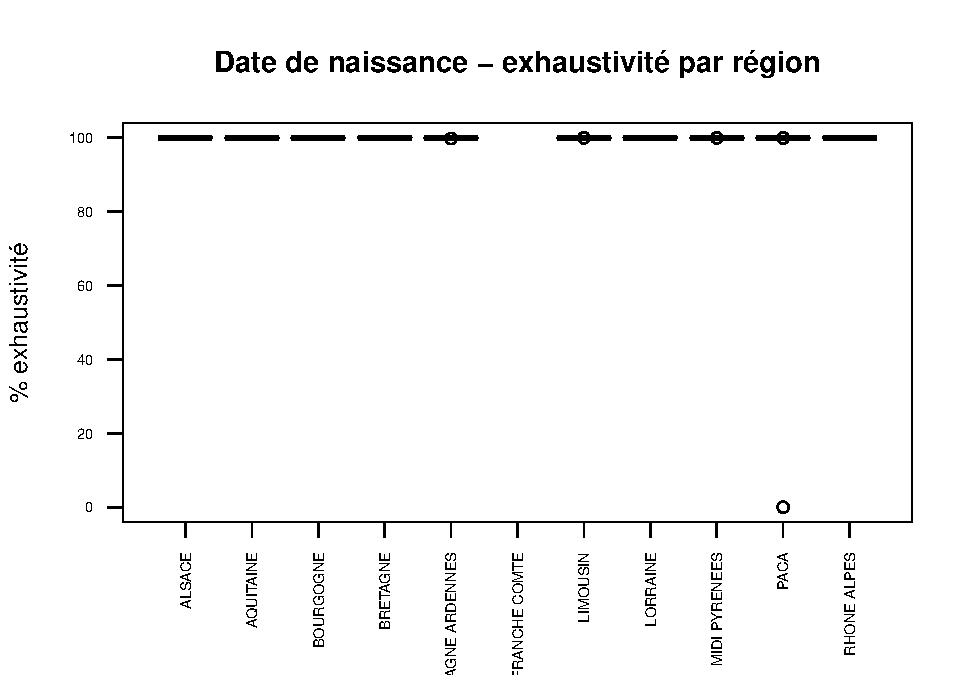
\includegraphics{septembre2015_files/figure-latex/unnamed-chunk-35-1.pdf}

\subsection{Diagnostic (DP)}\label{diagnostic-dp-2}

\begin{verbatim}
                   Min Max moyenne médiane ecart.type Nb   Q25 Q75
ALSACE               0  99      52      52     33.870 29  18.0  86
AQUITAINE            0 100      63      84     39.785 35  27.3  96
BOURGOGNE            0 100      62      95     45.024 23   3.8  99
BRETAGNE             0 100      67      91     39.331 30  24.0  98
CHAMPAGNE ARDENNES   0 100      74      98     37.783 16  63.6  99
FRANCHE COMTE      100 100     100     100      0.028 13 100.0 100
LIMOUSIN            86  99      97      98      4.257  9  97.6  99
LORRAINE            33 100      96     100     13.900 23  99.0 100
MIDI PYRENEES        0 100      71      92     37.820 74  35.4  98
PACA                 0 100      89      98     23.628 50  92.9  98
RHONE ALPES          0 100      72      92     36.685 70  66.0  96
\end{verbatim}

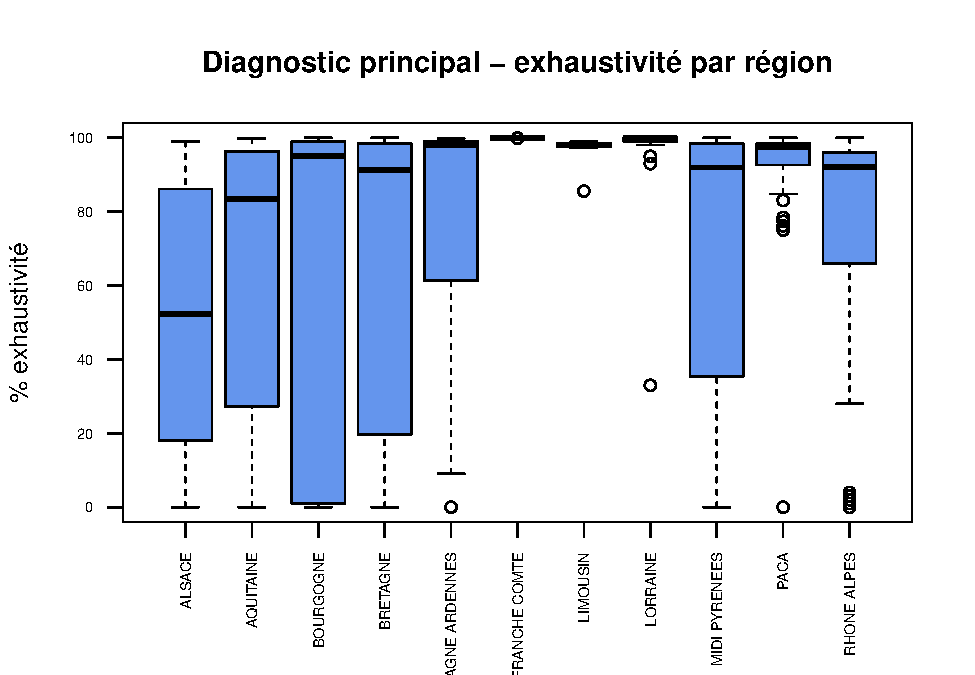
\includegraphics{septembre2015_files/figure-latex/unnamed-chunk-36-1.pdf}
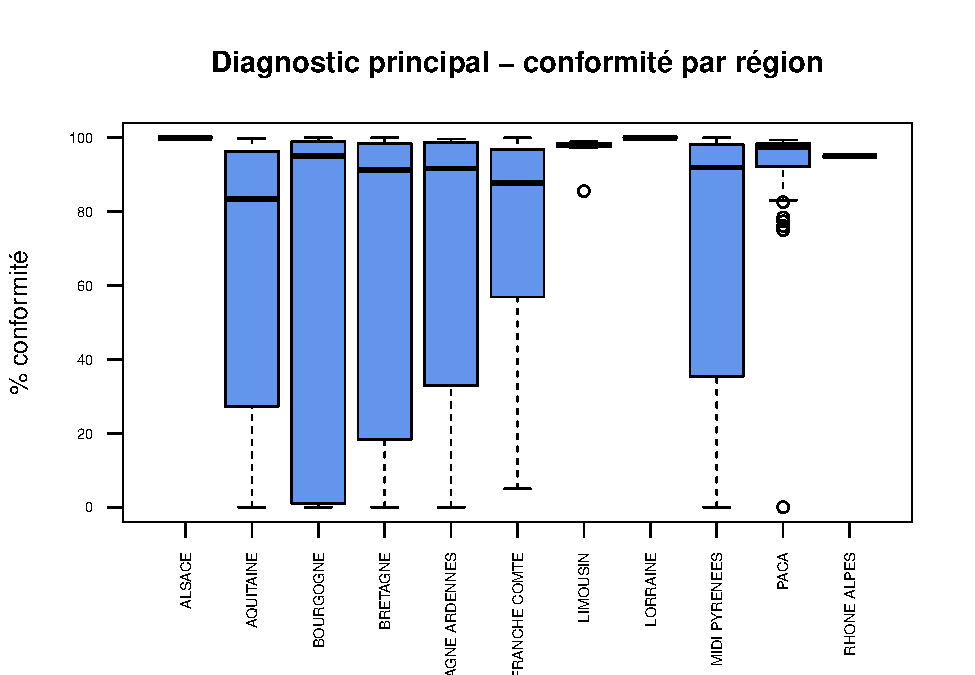
\includegraphics{septembre2015_files/figure-latex/unnamed-chunk-36-2.pdf}

\subsection{Mode de sortie (MS)}\label{mode-de-sortie-ms-2}

\begin{verbatim}
                    Min Max moyenne médiane ecart.type Nb Q25 Q75
ALSACE             15.7 100      70      84      32.61 29  30  96
AQUITAINE           0.0 100      89     100      27.60 35  98 100
BOURGOGNE           0.0 100      81     100      39.19 23  97 100
BRETAGNE           13.5 100      92      99      21.62 30  98 100
CHAMPAGNE ARDENNES 69.1 100      95     100       9.62 16  96 100
FRANCHE COMTE       4.9  99      73      87      30.54 13  57  97
LIMOUSIN           99.4 100     100     100       0.22  9 100 100
LORRAINE           98.0  99      99      99       0.21 23  99  99
MIDI PYRENEES       0.0 100      93     100      18.94 74  98 100
PACA                0.0 100      87     100      29.08 50  94 100
RHONE ALPES         0.0 100      87     100      31.72 70  97 100
\end{verbatim}

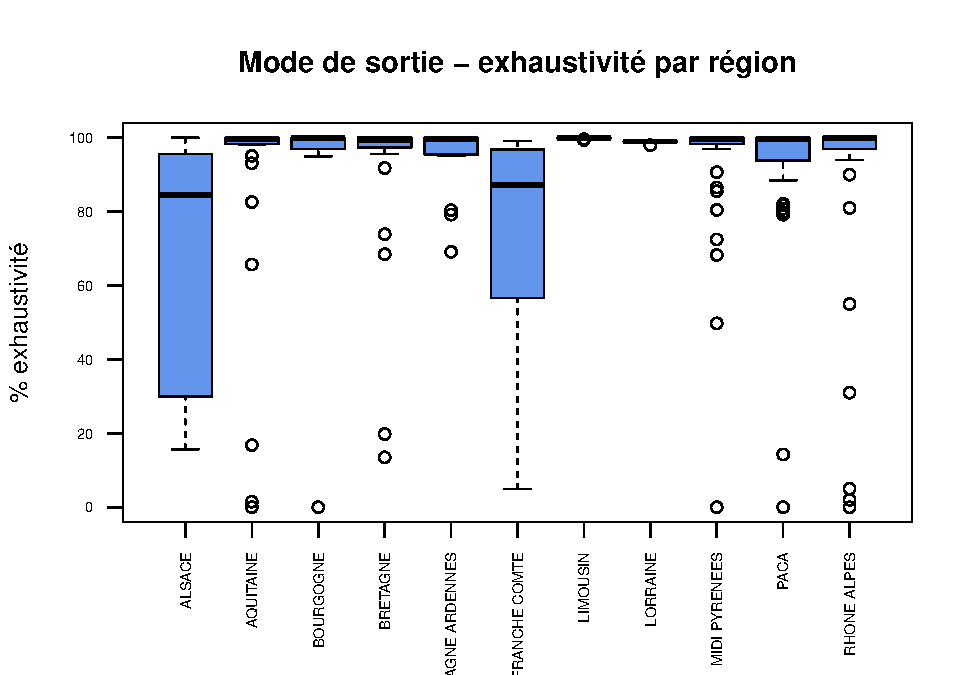
\includegraphics{septembre2015_files/figure-latex/unnamed-chunk-37-1.pdf}
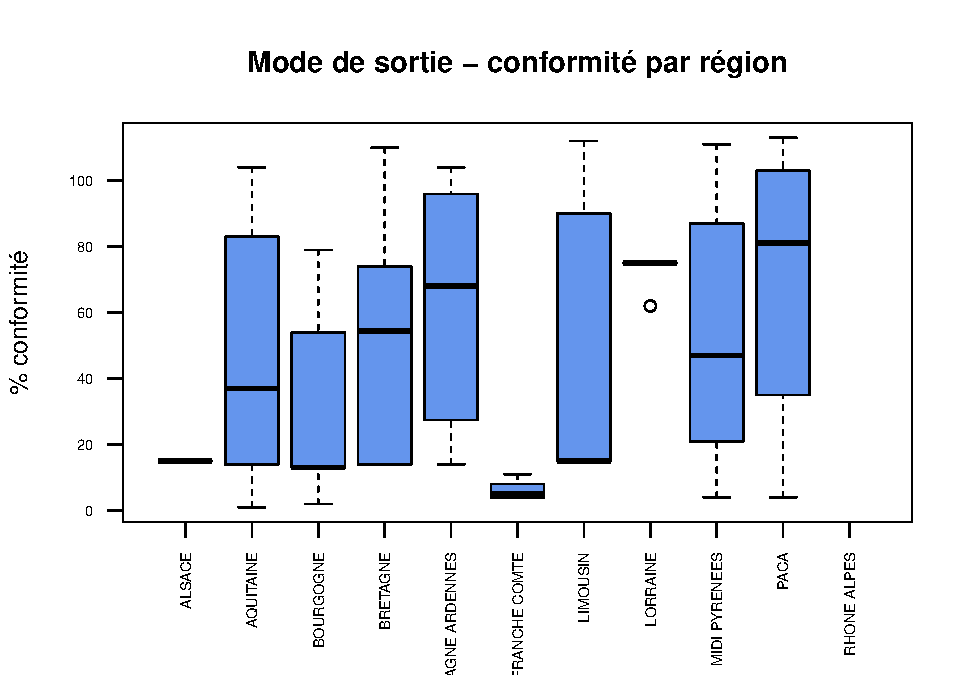
\includegraphics{septembre2015_files/figure-latex/unnamed-chunk-37-2.pdf}

\section{Résultats secondaires}\label{resultats-secondaires}

\subsection{\% de SU ne faisant pas de remontée de
RPU}\label{de-su-ne-faisant-pas-de-remontee-de-rpu}

\begin{verbatim}

NON OUI 
 17 355 
\end{verbatim}

\textless{}\textless{}\textless{}\textless{}\textless{}\textless{}\textless{}
HEAD
\textless{}\textless{}\textless{}\textless{}\textless{}\textless{}\textless{}
HEAD Messges pour les éditeurs, la DGOS, les DSI qui est responsable de
quoi ? intégration systématique des thésaurus, démarche d'amélioration.
Information proactive des sociétés savantes pour la publicationn des
Référentiels: info systématique de la Fedoru. Focaliser sur les
rectangles bleus. Voir si le n° de version permet de discriminer les
urqual qui remntent de ceux qui remontent mal. ======= ======= - nombre
de SU ne transmettant pas de RPU: 4.57 \%

\begin{quote}
\begin{quote}
\begin{quote}
\begin{quote}
\begin{quote}
\begin{quote}
\begin{quote}
d3a4aec0bdf9b8c3fdf91ab1588ec7345659735c Messages:
\end{quote}
\end{quote}
\end{quote}
\end{quote}
\end{quote}
\end{quote}
\end{quote}

\begin{itemize}
\tightlist
\item
  pour les éditeurs, la DGOS, les DSI qui est responsable de quoi ? DSI:
  de la saisie de l'info dans le SU à l'envoi des données à l'ORU:
  quelles sont les étapes de la chaîne de production
\item
  intégration systématique des thésaurus
\item
  quelle démarche d'amélioration.
\item
  Information proactive des sociétés savantes pour la publicationn des
  Référentiels: info systématique de la Fedoru.
\item
  Focaliser sur les rectangles bleus. Voir si le n° de version permet de
  discriminer les urqual qui remontent de ceux qui remontent mal.
  \textgreater{}\textgreater{}\textgreater{}\textgreater{}\textgreater{}\textgreater{}\textgreater{}
  b9052a7dd80e283494acc24d5348d639f959dc95
\end{itemize}

\section{Analyse de Urqual}\label{analyse-de-urqual}

\end{document}
